% Options for packages loaded elsewhere
\PassOptionsToPackage{unicode}{hyperref}
\PassOptionsToPackage{hyphens}{url}
%
\documentclass[
]{article}
\usepackage{amsmath,amssymb}
\usepackage{lmodern}
\usepackage{ifxetex,ifluatex}
\ifnum 0\ifxetex 1\fi\ifluatex 1\fi=0 % if pdftex
  \usepackage[T1]{fontenc}
  \usepackage[utf8]{inputenc}
  \usepackage{textcomp} % provide euro and other symbols
\else % if luatex or xetex
  \usepackage{unicode-math}
  \defaultfontfeatures{Scale=MatchLowercase}
  \defaultfontfeatures[\rmfamily]{Ligatures=TeX,Scale=1}
\fi
% Use upquote if available, for straight quotes in verbatim environments
\IfFileExists{upquote.sty}{\usepackage{upquote}}{}
\IfFileExists{microtype.sty}{% use microtype if available
  \usepackage[]{microtype}
  \UseMicrotypeSet[protrusion]{basicmath} % disable protrusion for tt fonts
}{}
\makeatletter
\@ifundefined{KOMAClassName}{% if non-KOMA class
  \IfFileExists{parskip.sty}{%
    \usepackage{parskip}
  }{% else
    \setlength{\parindent}{0pt}
    \setlength{\parskip}{6pt plus 2pt minus 1pt}}
}{% if KOMA class
  \KOMAoptions{parskip=half}}
\makeatother
\usepackage{xcolor}
\IfFileExists{xurl.sty}{\usepackage{xurl}}{} % add URL line breaks if available
\IfFileExists{bookmark.sty}{\usepackage{bookmark}}{\usepackage{hyperref}}
\hypersetup{
  pdftitle={Automation Explorations},
  hidelinks,
  pdfcreator={LaTeX via pandoc}}
\urlstyle{same} % disable monospaced font for URLs
\usepackage[margin=1in]{geometry}
\usepackage{color}
\usepackage{fancyvrb}
\newcommand{\VerbBar}{|}
\newcommand{\VERB}{\Verb[commandchars=\\\{\}]}
\DefineVerbatimEnvironment{Highlighting}{Verbatim}{commandchars=\\\{\}}
% Add ',fontsize=\small' for more characters per line
\usepackage{framed}
\definecolor{shadecolor}{RGB}{248,248,248}
\newenvironment{Shaded}{\begin{snugshade}}{\end{snugshade}}
\newcommand{\AlertTok}[1]{\textcolor[rgb]{0.94,0.16,0.16}{#1}}
\newcommand{\AnnotationTok}[1]{\textcolor[rgb]{0.56,0.35,0.01}{\textbf{\textit{#1}}}}
\newcommand{\AttributeTok}[1]{\textcolor[rgb]{0.77,0.63,0.00}{#1}}
\newcommand{\BaseNTok}[1]{\textcolor[rgb]{0.00,0.00,0.81}{#1}}
\newcommand{\BuiltInTok}[1]{#1}
\newcommand{\CharTok}[1]{\textcolor[rgb]{0.31,0.60,0.02}{#1}}
\newcommand{\CommentTok}[1]{\textcolor[rgb]{0.56,0.35,0.01}{\textit{#1}}}
\newcommand{\CommentVarTok}[1]{\textcolor[rgb]{0.56,0.35,0.01}{\textbf{\textit{#1}}}}
\newcommand{\ConstantTok}[1]{\textcolor[rgb]{0.00,0.00,0.00}{#1}}
\newcommand{\ControlFlowTok}[1]{\textcolor[rgb]{0.13,0.29,0.53}{\textbf{#1}}}
\newcommand{\DataTypeTok}[1]{\textcolor[rgb]{0.13,0.29,0.53}{#1}}
\newcommand{\DecValTok}[1]{\textcolor[rgb]{0.00,0.00,0.81}{#1}}
\newcommand{\DocumentationTok}[1]{\textcolor[rgb]{0.56,0.35,0.01}{\textbf{\textit{#1}}}}
\newcommand{\ErrorTok}[1]{\textcolor[rgb]{0.64,0.00,0.00}{\textbf{#1}}}
\newcommand{\ExtensionTok}[1]{#1}
\newcommand{\FloatTok}[1]{\textcolor[rgb]{0.00,0.00,0.81}{#1}}
\newcommand{\FunctionTok}[1]{\textcolor[rgb]{0.00,0.00,0.00}{#1}}
\newcommand{\ImportTok}[1]{#1}
\newcommand{\InformationTok}[1]{\textcolor[rgb]{0.56,0.35,0.01}{\textbf{\textit{#1}}}}
\newcommand{\KeywordTok}[1]{\textcolor[rgb]{0.13,0.29,0.53}{\textbf{#1}}}
\newcommand{\NormalTok}[1]{#1}
\newcommand{\OperatorTok}[1]{\textcolor[rgb]{0.81,0.36,0.00}{\textbf{#1}}}
\newcommand{\OtherTok}[1]{\textcolor[rgb]{0.56,0.35,0.01}{#1}}
\newcommand{\PreprocessorTok}[1]{\textcolor[rgb]{0.56,0.35,0.01}{\textit{#1}}}
\newcommand{\RegionMarkerTok}[1]{#1}
\newcommand{\SpecialCharTok}[1]{\textcolor[rgb]{0.00,0.00,0.00}{#1}}
\newcommand{\SpecialStringTok}[1]{\textcolor[rgb]{0.31,0.60,0.02}{#1}}
\newcommand{\StringTok}[1]{\textcolor[rgb]{0.31,0.60,0.02}{#1}}
\newcommand{\VariableTok}[1]{\textcolor[rgb]{0.00,0.00,0.00}{#1}}
\newcommand{\VerbatimStringTok}[1]{\textcolor[rgb]{0.31,0.60,0.02}{#1}}
\newcommand{\WarningTok}[1]{\textcolor[rgb]{0.56,0.35,0.01}{\textbf{\textit{#1}}}}
\usepackage{graphicx}
\makeatletter
\def\maxwidth{\ifdim\Gin@nat@width>\linewidth\linewidth\else\Gin@nat@width\fi}
\def\maxheight{\ifdim\Gin@nat@height>\textheight\textheight\else\Gin@nat@height\fi}
\makeatother
% Scale images if necessary, so that they will not overflow the page
% margins by default, and it is still possible to overwrite the defaults
% using explicit options in \includegraphics[width, height, ...]{}
\setkeys{Gin}{width=\maxwidth,height=\maxheight,keepaspectratio}
% Set default figure placement to htbp
\makeatletter
\def\fps@figure{htbp}
\makeatother
\setlength{\emergencystretch}{3em} % prevent overfull lines
\providecommand{\tightlist}{%
  \setlength{\itemsep}{0pt}\setlength{\parskip}{0pt}}
\setcounter{secnumdepth}{-\maxdimen} % remove section numbering
\ifluatex
  \usepackage{selnolig}  % disable illegal ligatures
\fi

\title{Automation Explorations}
\author{}
\date{\vspace{-2.5em}}

\begin{document}
\maketitle

In this section we explore attempting to find the sub arrays
automatically and then the features within them (i.e.~pad centres
adjusted to peak points). So the main goal it to find the sub array
locations and fine adjustments within them.

This report section was generated using RMarkdown in RStudio with the
\href{https://rstudio.github.io/reticulate/index.html}{r-reticulate}
package to support Python sections. The included script generates the
figures.

I used this project to also learn Python (so don't judge the code
elements :) ).

I have included the code for your interest but hidden it by default to
improve readability.

I have tried to leave in `failures' so you can see how the thought
processes progressed.

The `automation' will be highly tuned to image 488 but the chosen
processes will try to avoid over customisation (e.g.~use gradient info
rather than grey level thresholds etc.)

\hypertarget{analysis}{%
\section{Analysis}\label{analysis}}

First we want to reliably find the sub arrays background thinking is
based on two approaches:

\begin{itemize}
\tightlist
\item
  quickly try and find the bulk of the pad features and use the
  coordinates to estimate sub array locations, or
\item
  use global image transforms to find the sub array boundaries
  e.g.~pyramid decomposition, edge detectors, blurring.
\end{itemize}

Generally we will just try a few approaches and look at the results and
build from there.

\hypertarget{python-library-setup}{%
\subsubsection{Python library Setup}\label{python-library-setup}}

The libraries used in this analysis.

We are using additional libraries here

\href{https://scikit-image.org/}{\includegraphics[width=0.2\textwidth,height=\textheight]{https://scikit-image.org/_static/img/logo.png}}
and \href{https://pywavelets.readthedocs.io}{PyWavelets - Wavelet
Transforms in Python}

\begin{Shaded}
\begin{Highlighting}[]
\ImportTok{import}\NormalTok{ cv2 }\ImportTok{as}\NormalTok{ cv}
\ImportTok{import}\NormalTok{ numpy }\ImportTok{as}\NormalTok{ np}
\ImportTok{from}\NormalTok{ matplotlib }\ImportTok{import}\NormalTok{ pyplot }\ImportTok{as}\NormalTok{ plt}
\ImportTok{import}\NormalTok{ pywt}
\ImportTok{import}\NormalTok{ matplotlib.colors }\ImportTok{as}\NormalTok{ colors}

\ImportTok{from}\NormalTok{ matplotlib }\ImportTok{import}\NormalTok{ cm}
\ImportTok{from}\NormalTok{ math }\ImportTok{import}\NormalTok{ sqrt}
\ImportTok{from}\NormalTok{ skimage.feature }\ImportTok{import}\NormalTok{ blob\_dog, blob\_log, blob\_doh}

\CommentTok{\#plt.rcParams["figure.figsize"] = (20,13)}

\CommentTok{\# Simple rowMultiplication used in pad }
\KeywordTok{def}\NormalTok{ rowMult(Mat,theRow,xv,yv):}
    \ControlFlowTok{return}\NormalTok{(Mat[theRow,}\DecValTok{0}\NormalTok{]}\OperatorTok{*}\NormalTok{xv}\OperatorTok{+}\NormalTok{Mat[theRow,}\DecValTok{1}\NormalTok{]}\OperatorTok{*}\NormalTok{yv}\OperatorTok{+}\NormalTok{Mat[theRow,}\DecValTok{2}\NormalTok{])}

\KeywordTok{def}\NormalTok{ gridBorders(theSums,perc):}
\NormalTok{  percen}\OperatorTok{=}\NormalTok{np.percentile(theSums,perc)}
\NormalTok{  matchingX}\OperatorTok{=}\NormalTok{np.arange(}\DecValTok{0}\NormalTok{,}\BuiltInTok{len}\NormalTok{(theSums))[theSums}\OperatorTok{\textless{}}\NormalTok{percen]}
\NormalTok{  arr}\OperatorTok{=}\NormalTok{np.array(matchingX[}\DecValTok{0}\NormalTok{])}
  \ControlFlowTok{for}\NormalTok{ i }\KeywordTok{in}\NormalTok{ np.arange(}\DecValTok{1}\NormalTok{,}\BuiltInTok{len}\NormalTok{(matchingX)):}
    \ControlFlowTok{if}\NormalTok{ matchingX[i]}\OperatorTok{{-}}\NormalTok{matchingX[i}\OperatorTok{{-}}\DecValTok{1}\NormalTok{]}\OperatorTok{!=}\DecValTok{1}\NormalTok{:}
\NormalTok{      arr}\OperatorTok{=}\NormalTok{np.append(arr,[matchingX[i}\OperatorTok{{-}}\DecValTok{1}\NormalTok{],matchingX[i]])}
\NormalTok{  arr}\OperatorTok{=}\NormalTok{np.append(arr,matchingX[i])}
  \ControlFlowTok{return}\NormalTok{(arr)}

\NormalTok{folderStub}\OperatorTok{=}\StringTok{"procimage/"} \CommentTok{\# enable detailed review in a image review tool}
\NormalTok{scaleFac}\OperatorTok{=}\DecValTok{4} \CommentTok{\# how much the subAreas are zoomed }
\end{Highlighting}
\end{Shaded}

\hypertarget{manually-assessed-parameters}{%
\subsubsection{Manually assessed
parameters}\label{manually-assessed-parameters}}

These are the parameters used in the geometric analysis analysis. They
came from looking at the 488 image in an imaging tool and noting pixel
coordinates.

We will use the pad estimates here in the algorithms but the patch
information will just be used as a reference as we are going to try and
seek them automatically.

\begin{Shaded}
\begin{Highlighting}[]

\NormalTok{numPads}\OperatorTok{=}\DecValTok{123} \CommentTok{\# got this from counting peaks in a subArea. image 488}
\NormalTok{interpad}\OperatorTok{=}\DecValTok{5}  \CommentTok{\# got this from measuring between peaks in a subArea. image 488}

\CommentTok{\# TL,TR,BR,BL}
\CommentTok{\# manually selected from 488 image}
\NormalTok{patches}\OperatorTok{=}\NormalTok{\{}
\StringTok{"Patch 1"}\NormalTok{:np.array([[}\DecValTok{461}\NormalTok{,}\DecValTok{621}\NormalTok{],[}\DecValTok{1082}\NormalTok{,}\DecValTok{625}\NormalTok{],[}\DecValTok{1077}\NormalTok{,}\DecValTok{1246}\NormalTok{],[}\DecValTok{457}\NormalTok{,}\DecValTok{1241}\NormalTok{]],np.int32),}
\StringTok{"Patch 2"}\NormalTok{:np.array([[}\DecValTok{1150}\NormalTok{,}\DecValTok{626}\NormalTok{],[}\DecValTok{1771}\NormalTok{,}\DecValTok{630}\NormalTok{],[}\DecValTok{1767}\NormalTok{,}\DecValTok{1252}\NormalTok{],[}\DecValTok{1145}\NormalTok{,}\DecValTok{1246}\NormalTok{]],np.int32),}
\StringTok{"Patch 3"}\NormalTok{:np.array([[}\DecValTok{456}\NormalTok{,}\DecValTok{1310}\NormalTok{],[}\DecValTok{1077}\NormalTok{,}\DecValTok{1314}\NormalTok{],[}\DecValTok{1072}\NormalTok{,}\DecValTok{1935}\NormalTok{],[}\DecValTok{450}\NormalTok{,}\DecValTok{1932}\NormalTok{]],np.int32),}
\StringTok{"Patch 4"}\NormalTok{:np.array([[}\DecValTok{1145}\NormalTok{,}\DecValTok{1315}\NormalTok{],[}\DecValTok{1766}\NormalTok{,}\DecValTok{1319}\NormalTok{],[}\DecValTok{1763}\NormalTok{,}\DecValTok{1942}\NormalTok{],[}\DecValTok{1141}\NormalTok{,}\DecValTok{1936}\NormalTok{]],np.int32)}
\NormalTok{\}}
\end{Highlighting}
\end{Shaded}

\hypertarget{loading-and-contrast-stretching}{%
\subsubsection{Loading and contrast
stretching}\label{loading-and-contrast-stretching}}

I am used to viewing black features on a white background so the images
are loaded inverted and contrast stretched for viewing. The original 16
bit image is also retained for measurements in feature areas.

\hypertarget{guess-where-the-sub-arrays-may-be}{%
\subsubsection{Guess where the sub arrays may
be}\label{guess-where-the-sub-arrays-may-be}}

The basic review showed that in the 488 image at least the background
between the arrays is lower so here we explore a quick and easy way to
obtain a `ball park' estimate which we then could use template matching
or a similar approach to derive accurate array edge points instead of
the manually supplied ones.

All we are doing is creating a sum of the pixels columns (blue) and then
rows (orange). The horizontal green lines mark percentiles of the column
sums (we use it to choose a threshold). The vertical red and purple
lines are the boundaries that result which are then displayed in cyan on
the image.

\begin{Shaded}
\begin{Highlighting}[]

\CommentTok{\# take a guess where the inter subarray regions are based on grey level values}
\NormalTok{threshPerc}\OperatorTok{=}\DecValTok{8}
\NormalTok{colSums}\OperatorTok{=}\NormalTok{ origimg.}\BuiltInTok{sum}\NormalTok{(axis}\OperatorTok{=}\DecValTok{0}\NormalTok{)}
\NormalTok{rowSums}\OperatorTok{=}\NormalTok{ origimg.}\BuiltInTok{sum}\NormalTok{(axis}\OperatorTok{=}\DecValTok{1}\NormalTok{)}
\NormalTok{percen}\OperatorTok{=}\NormalTok{np.percentile(colSums,(}\DecValTok{9}\NormalTok{,}\DecValTok{10}\NormalTok{,}\DecValTok{20}\NormalTok{,}\DecValTok{30}\NormalTok{,}\DecValTok{40}\NormalTok{,}\DecValTok{50}\NormalTok{,}\DecValTok{60}\NormalTok{,}\DecValTok{70}\NormalTok{,}\DecValTok{80}\NormalTok{))}
\NormalTok{arrX}\OperatorTok{=}\NormalTok{gridBorders(colSums,threshPerc)}
\NormalTok{arrY}\OperatorTok{=}\NormalTok{gridBorders(rowSums,threshPerc)}


\CommentTok{\#plt.ioff();}
\NormalTok{plt.plot(np.arange(}\DecValTok{0}\NormalTok{,}\BuiltInTok{len}\NormalTok{(colSums)),colSums)}\OperatorTok{;}
\NormalTok{plt.plot(np.arange(}\DecValTok{0}\NormalTok{,}\BuiltInTok{len}\NormalTok{(rowSums)),rowSums)}\OperatorTok{;}
\NormalTok{plt.vlines(arrX,}\DecValTok{0}\NormalTok{,percen[}\DecValTok{8}\NormalTok{],colors}\OperatorTok{=}\NormalTok{np.repeat(}\StringTok{\textquotesingle{}r\textquotesingle{}}\NormalTok{,}\BuiltInTok{len}\NormalTok{(arrX)))}\OperatorTok{;}
\NormalTok{plt.vlines(arrY,}\DecValTok{0}\NormalTok{,percen[}\DecValTok{8}\NormalTok{],colors}\OperatorTok{=}\NormalTok{np.repeat(}\StringTok{\textquotesingle{}purple\textquotesingle{}}\NormalTok{,}\BuiltInTok{len}\NormalTok{(arrY)))}\OperatorTok{;}
\NormalTok{plt.hlines(percen,}\DecValTok{0}\NormalTok{,}\BuiltInTok{len}\NormalTok{(colSums),}\StringTok{\textquotesingle{}g\textquotesingle{}}\NormalTok{)}\OperatorTok{;}
\NormalTok{plt.grid(}\VariableTok{True}\NormalTok{)}\OperatorTok{;}
\NormalTok{plt.show()}
\end{Highlighting}
\end{Shaded}


\includegraphics{Auto_files/figure-latex/unnamed-chunk-1-1.pdf}

\begin{Shaded}
\begin{Highlighting}[]
\CommentTok{\# draw them on the image}
\ControlFlowTok{for}\NormalTok{ i }\KeywordTok{in}\NormalTok{ np.arange(}\DecValTok{0}\NormalTok{,}\BuiltInTok{len}\NormalTok{(arrX),}\DecValTok{2}\NormalTok{):}
\NormalTok{  colimg}\OperatorTok{=}\NormalTok{cv.rectangle(colimg,(arrX[i],}\DecValTok{0}\NormalTok{),(arrX[i}\OperatorTok{+}\DecValTok{1}\NormalTok{],colimg.shape[}\DecValTok{1}\NormalTok{]),(}\DecValTok{65535}\NormalTok{,}\DecValTok{65535}\NormalTok{,}\DecValTok{0}\NormalTok{),}\DecValTok{1}\NormalTok{)}
  
\ControlFlowTok{for}\NormalTok{ i }\KeywordTok{in}\NormalTok{ np.arange(}\DecValTok{0}\NormalTok{,}\BuiltInTok{len}\NormalTok{(arrY),}\DecValTok{2}\NormalTok{):}
\NormalTok{  colimg}\OperatorTok{=}\NormalTok{cv.rectangle(colimg,(}\DecValTok{0}\NormalTok{,arrY[i]),(colimg.shape[}\DecValTok{0}\NormalTok{],arrY[i}\OperatorTok{+}\DecValTok{1}\NormalTok{]),(}\DecValTok{65535}\NormalTok{,}\DecValTok{65535}\NormalTok{,}\DecValTok{0}\NormalTok{),}\DecValTok{1}\NormalTok{)}
  
\CommentTok{\# Draw the manually defined patches on too}
\ControlFlowTok{for}\NormalTok{ patchName }\KeywordTok{in}\NormalTok{ patches:}
\NormalTok{    pts}\OperatorTok{=}\NormalTok{patches[patchName]}

\NormalTok{    colimg}\OperatorTok{=}\NormalTok{cv.polylines(colimg,[pts.reshape((}\OperatorTok{{-}}\DecValTok{1}\NormalTok{,}\DecValTok{1}\NormalTok{,}\DecValTok{2}\NormalTok{))],}\VariableTok{True}\NormalTok{,(}\DecValTok{65535}\NormalTok{,}\DecValTok{0}\NormalTok{,}\DecValTok{0}\NormalTok{))}
\NormalTok{    colimg}\OperatorTok{=}\NormalTok{cv.putText(colimg,patchName,(pts[}\DecValTok{0}\NormalTok{,}\DecValTok{0}\NormalTok{],pts[}\DecValTok{0}\NormalTok{,}\DecValTok{1}\NormalTok{]}\OperatorTok{{-}}\DecValTok{2}\OperatorTok{*}\NormalTok{interpad),cv.FONT\_HERSHEY\_SIMPLEX,}\DecValTok{1}\NormalTok{,(}\DecValTok{65535}\NormalTok{,}\DecValTok{0}\NormalTok{,}\DecValTok{0}\NormalTok{),}\DecValTok{2}\NormalTok{,cv.LINE\_AA)}


\NormalTok{guessImageFile}\OperatorTok{=}\NormalTok{folderStub}\OperatorTok{+}\NormalTok{fileStub}\OperatorTok{+}\StringTok{" origGuess.png"}
\NormalTok{ok}\OperatorTok{=}\NormalTok{cv.imwrite(guessImageFile, colimg)}
\end{Highlighting}
\end{Shaded}

\begin{center}\includegraphics[width=1\linewidth]{procimage/im488 origGuess} \end{center}

View full image \href{procimage/im488\%20origGuess.png}{procimage/im488
origGuess.png}

\begin{Shaded}
\begin{Highlighting}[]


\NormalTok{laplacian }\OperatorTok{=}\NormalTok{ cv.Laplacian(img,cv.CV\_64F)}
\NormalTok{sobelx }\OperatorTok{=}\NormalTok{ cv.Sobel(img,cv.CV\_64F,}\DecValTok{1}\NormalTok{,}\DecValTok{0}\NormalTok{,ksize}\OperatorTok{=}\DecValTok{5}\NormalTok{)}
\NormalTok{sobely }\OperatorTok{=}\NormalTok{ cv.Sobel(img,cv.CV\_64F,}\DecValTok{0}\NormalTok{,}\DecValTok{1}\NormalTok{,ksize}\OperatorTok{=}\DecValTok{5}\NormalTok{)}
\NormalTok{plt.subplot(}\DecValTok{2}\NormalTok{,}\DecValTok{2}\NormalTok{,}\DecValTok{1}\NormalTok{)}\OperatorTok{;}\NormalTok{plt.imshow(img,cmap }\OperatorTok{=} \StringTok{\textquotesingle{}gray\textquotesingle{}}\NormalTok{)}\OperatorTok{;}
\NormalTok{plt.title(}\StringTok{\textquotesingle{}Original\textquotesingle{}}\NormalTok{)}\OperatorTok{;}\NormalTok{ plt.xticks([])}\OperatorTok{;}\NormalTok{ plt.yticks([])}\OperatorTok{;}
\NormalTok{plt.subplot(}\DecValTok{2}\NormalTok{,}\DecValTok{2}\NormalTok{,}\DecValTok{2}\NormalTok{),plt.imshow(laplacian,cmap }\OperatorTok{=} \StringTok{\textquotesingle{}gray\textquotesingle{}}\NormalTok{)}\OperatorTok{;}
\NormalTok{plt.title(}\StringTok{\textquotesingle{}Laplacian\textquotesingle{}}\NormalTok{)}\OperatorTok{;}\NormalTok{ plt.xticks([])}\OperatorTok{;}\NormalTok{ plt.yticks([])}\OperatorTok{;}
\NormalTok{plt.subplot(}\DecValTok{2}\NormalTok{,}\DecValTok{2}\NormalTok{,}\DecValTok{3}\NormalTok{)}\OperatorTok{;}\NormalTok{plt.imshow(sobelx,cmap }\OperatorTok{=} \StringTok{\textquotesingle{}gray\textquotesingle{}}\NormalTok{)}\OperatorTok{;}
\NormalTok{plt.title(}\StringTok{\textquotesingle{}Sobel X\textquotesingle{}}\NormalTok{)}\OperatorTok{;}\NormalTok{ plt.xticks([])}\OperatorTok{;}\NormalTok{ plt.yticks([])}\OperatorTok{;}
\NormalTok{plt.subplot(}\DecValTok{2}\NormalTok{,}\DecValTok{2}\NormalTok{,}\DecValTok{4}\NormalTok{)}\OperatorTok{;}\NormalTok{plt.imshow(sobely,cmap }\OperatorTok{=} \StringTok{\textquotesingle{}gray\textquotesingle{}}\NormalTok{)}\OperatorTok{;}
\NormalTok{plt.title(}\StringTok{\textquotesingle{}Sobel Y\textquotesingle{}}\NormalTok{)}\OperatorTok{;}\NormalTok{ plt.xticks([])}\OperatorTok{;}\NormalTok{ plt.yticks([])}\OperatorTok{;}
\NormalTok{plt.show()}
\end{Highlighting}
\end{Shaded}


\includegraphics{Auto_files/figure-latex/unnamed-chunk-1-1.pdf}

\begin{Shaded}
\begin{Highlighting}[]

\NormalTok{higherRes}\OperatorTok{=}\NormalTok{ img}
\NormalTok{lowerRes}\OperatorTok{=}\NormalTok{cv.pyrDown(higherRes)}

\ControlFlowTok{while}\NormalTok{ lowerRes.shape[}\DecValTok{0}\NormalTok{]}\OperatorTok{\textgreater{}}\DecValTok{64}\NormalTok{:}
\NormalTok{  lowerRes}\OperatorTok{=}\NormalTok{cv.pyrDown(higherRes)}
\NormalTok{  \_}\OperatorTok{=}\NormalTok{plt.imshow(lowerRes,cmap }\OperatorTok{=} \StringTok{\textquotesingle{}gray\textquotesingle{}}\NormalTok{)}\OperatorTok{;}
\NormalTok{  \_}\OperatorTok{=}\NormalTok{plt.title(}\StringTok{\textquotesingle{}Original \textquotesingle{}}\OperatorTok{+}\BuiltInTok{str}\NormalTok{(lowerRes.shape[}\DecValTok{0}\NormalTok{]))}\OperatorTok{;}\NormalTok{ plt.xticks([])}\OperatorTok{;}\NormalTok{ plt.yticks([])}\OperatorTok{;}
\NormalTok{  plt.show()}\OperatorTok{;}
  
\NormalTok{  laplacian }\OperatorTok{=}\NormalTok{ cv.Laplacian(lowerRes,cv.CV\_64F)}
\NormalTok{  \_}\OperatorTok{=}\NormalTok{plt.imshow(laplacian,cmap }\OperatorTok{=} \StringTok{\textquotesingle{}gray\textquotesingle{}}\NormalTok{)}\OperatorTok{;}
\NormalTok{  \_}\OperatorTok{=}\NormalTok{plt.title(}\StringTok{\textquotesingle{}Laplacian\textquotesingle{}}\OperatorTok{+}\BuiltInTok{str}\NormalTok{(laplacian.shape[}\DecValTok{0}\NormalTok{]))}\OperatorTok{;}\NormalTok{ plt.xticks([])}\OperatorTok{;}\NormalTok{ plt.yticks([])}\OperatorTok{;}
\NormalTok{  plt.show()}\OperatorTok{;}
\NormalTok{  higherRes}\OperatorTok{=}\NormalTok{lowerRes}
\end{Highlighting}
\end{Shaded}


\includegraphics{Auto_files/figure-latex/unnamed-chunk-1-3.pdf}

\includegraphics{Auto_files/figure-latex/unnamed-chunk-1-4.pdf}

\includegraphics{Auto_files/figure-latex/unnamed-chunk-1-5.pdf}

\includegraphics{Auto_files/figure-latex/unnamed-chunk-1-6.pdf}

\includegraphics{Auto_files/figure-latex/unnamed-chunk-1-7.pdf}
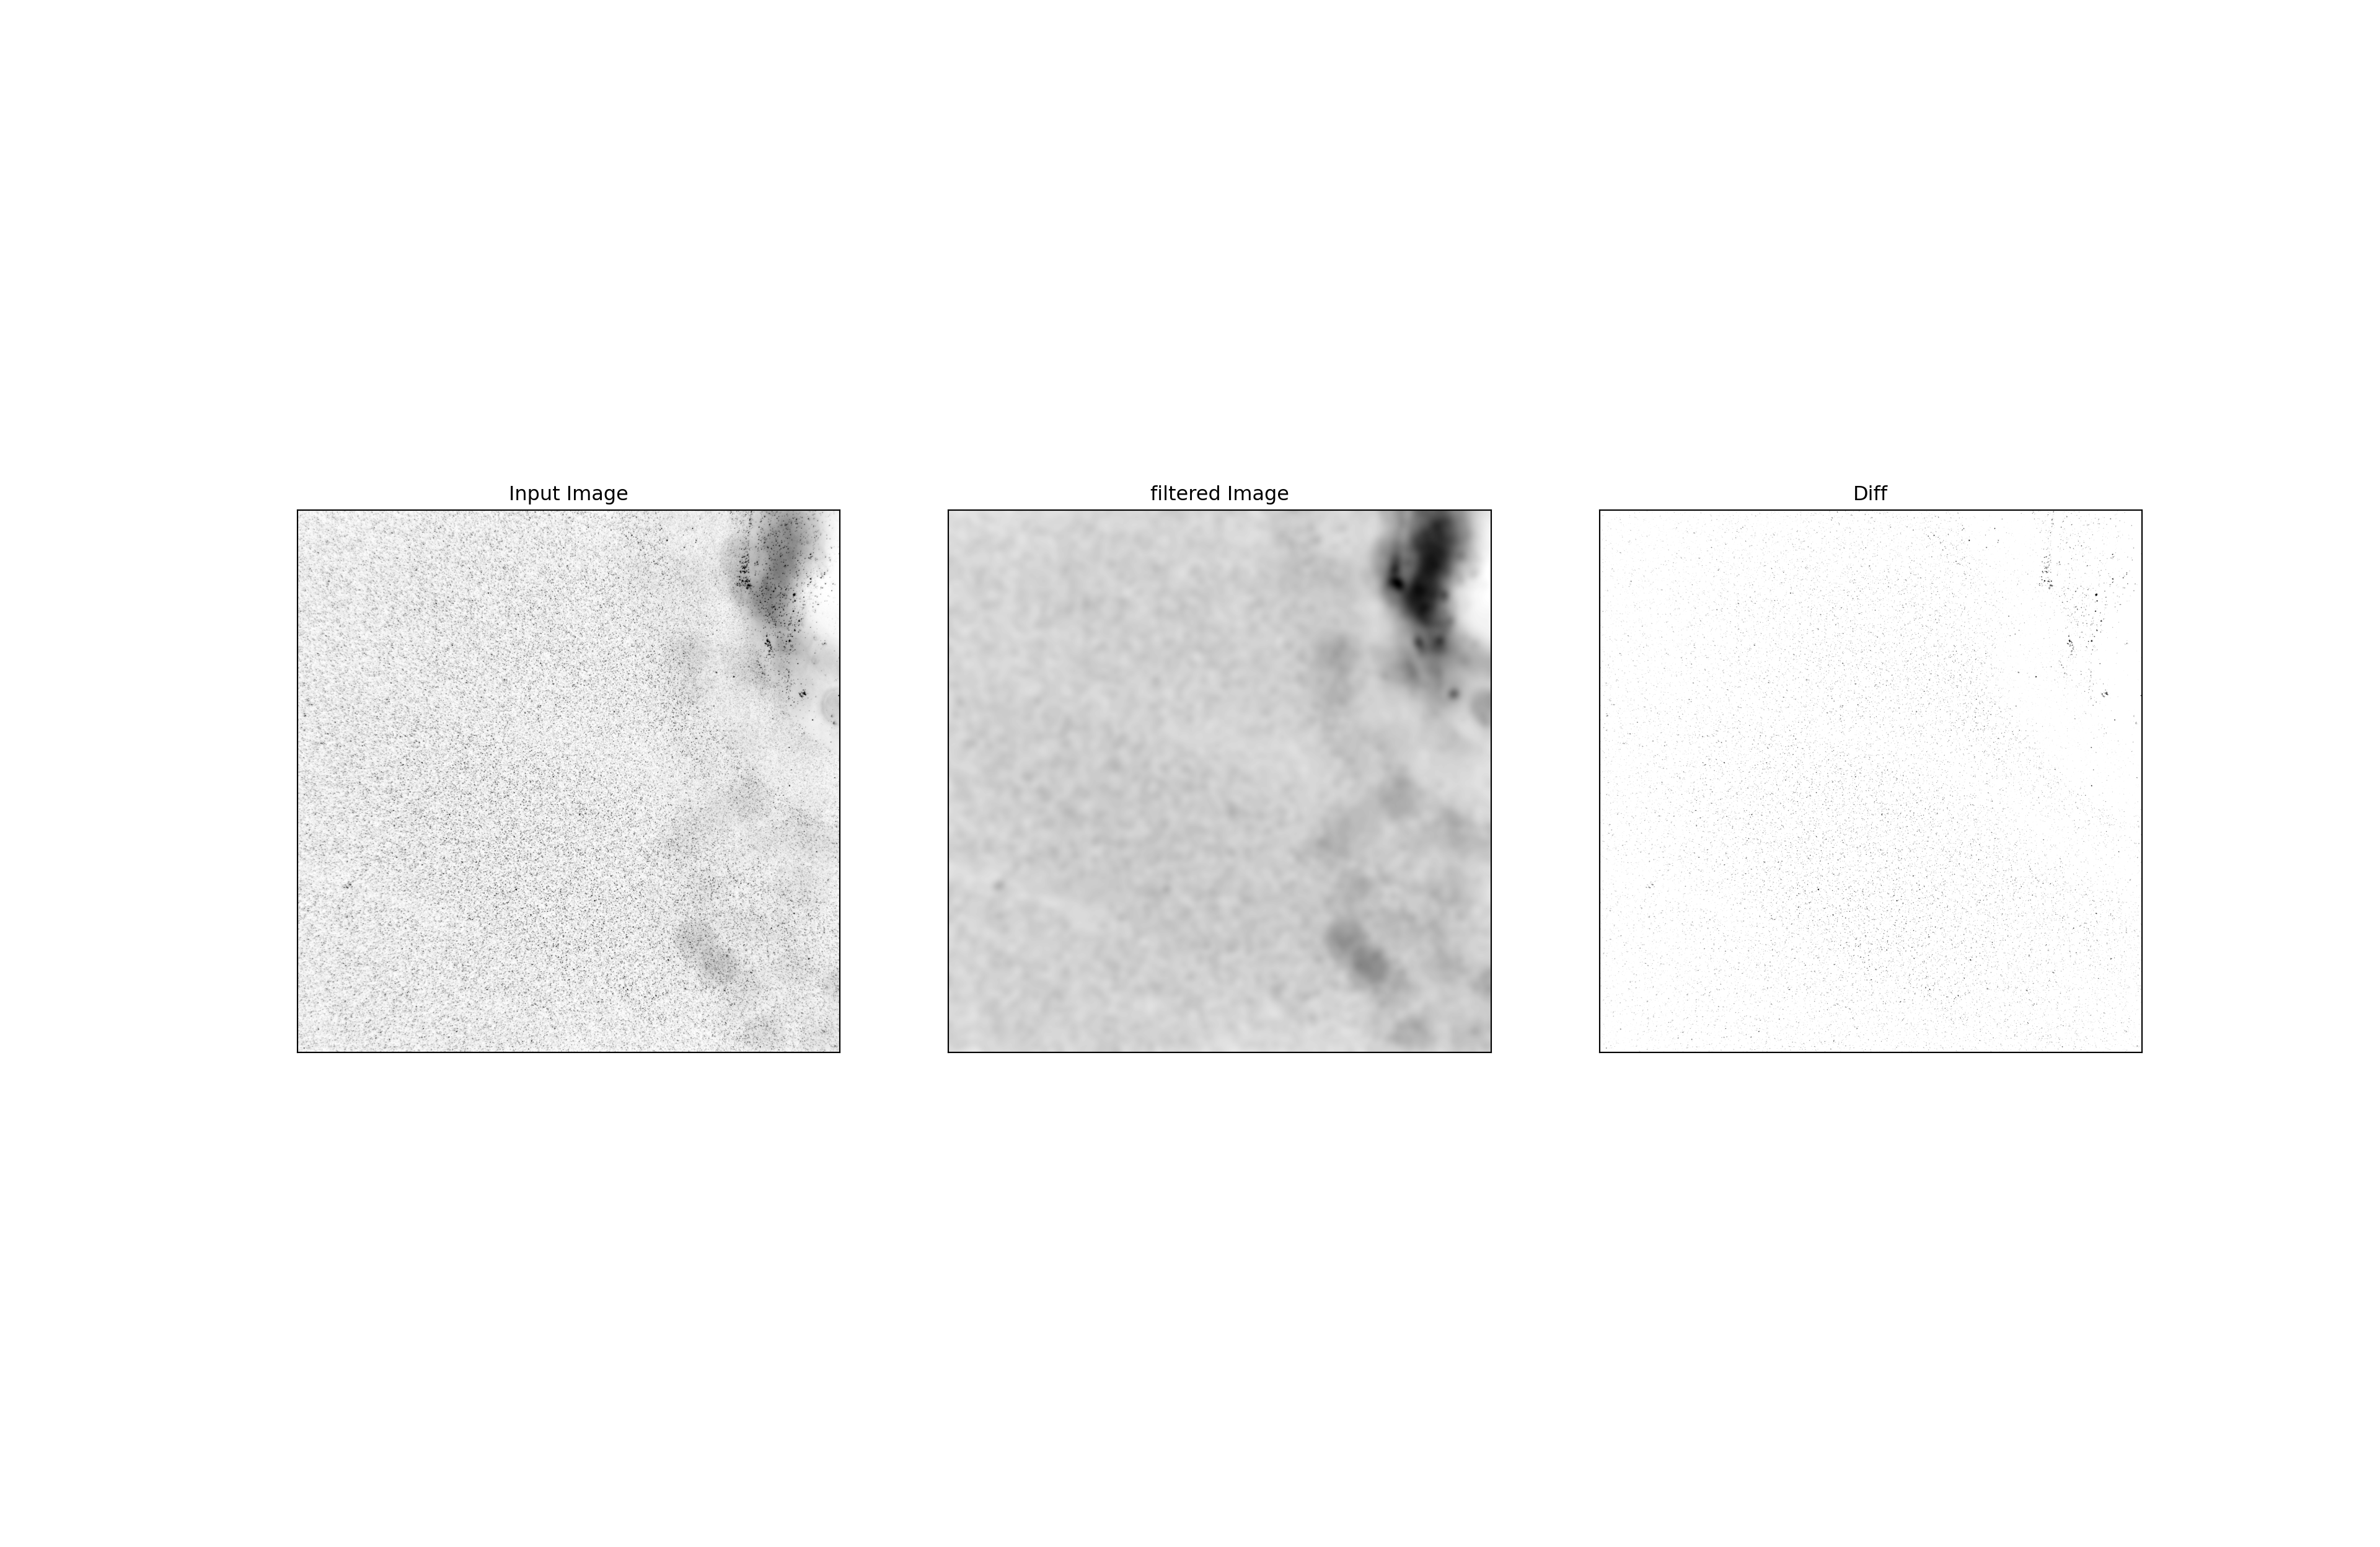
\includegraphics{Auto_files/figure-latex/unnamed-chunk-1-8.pdf}

\includegraphics{Auto_files/figure-latex/unnamed-chunk-1-9.pdf}

\includegraphics{Auto_files/figure-latex/unnamed-chunk-1-10.pdf}

\includegraphics{Auto_files/figure-latex/unnamed-chunk-1-11.pdf}
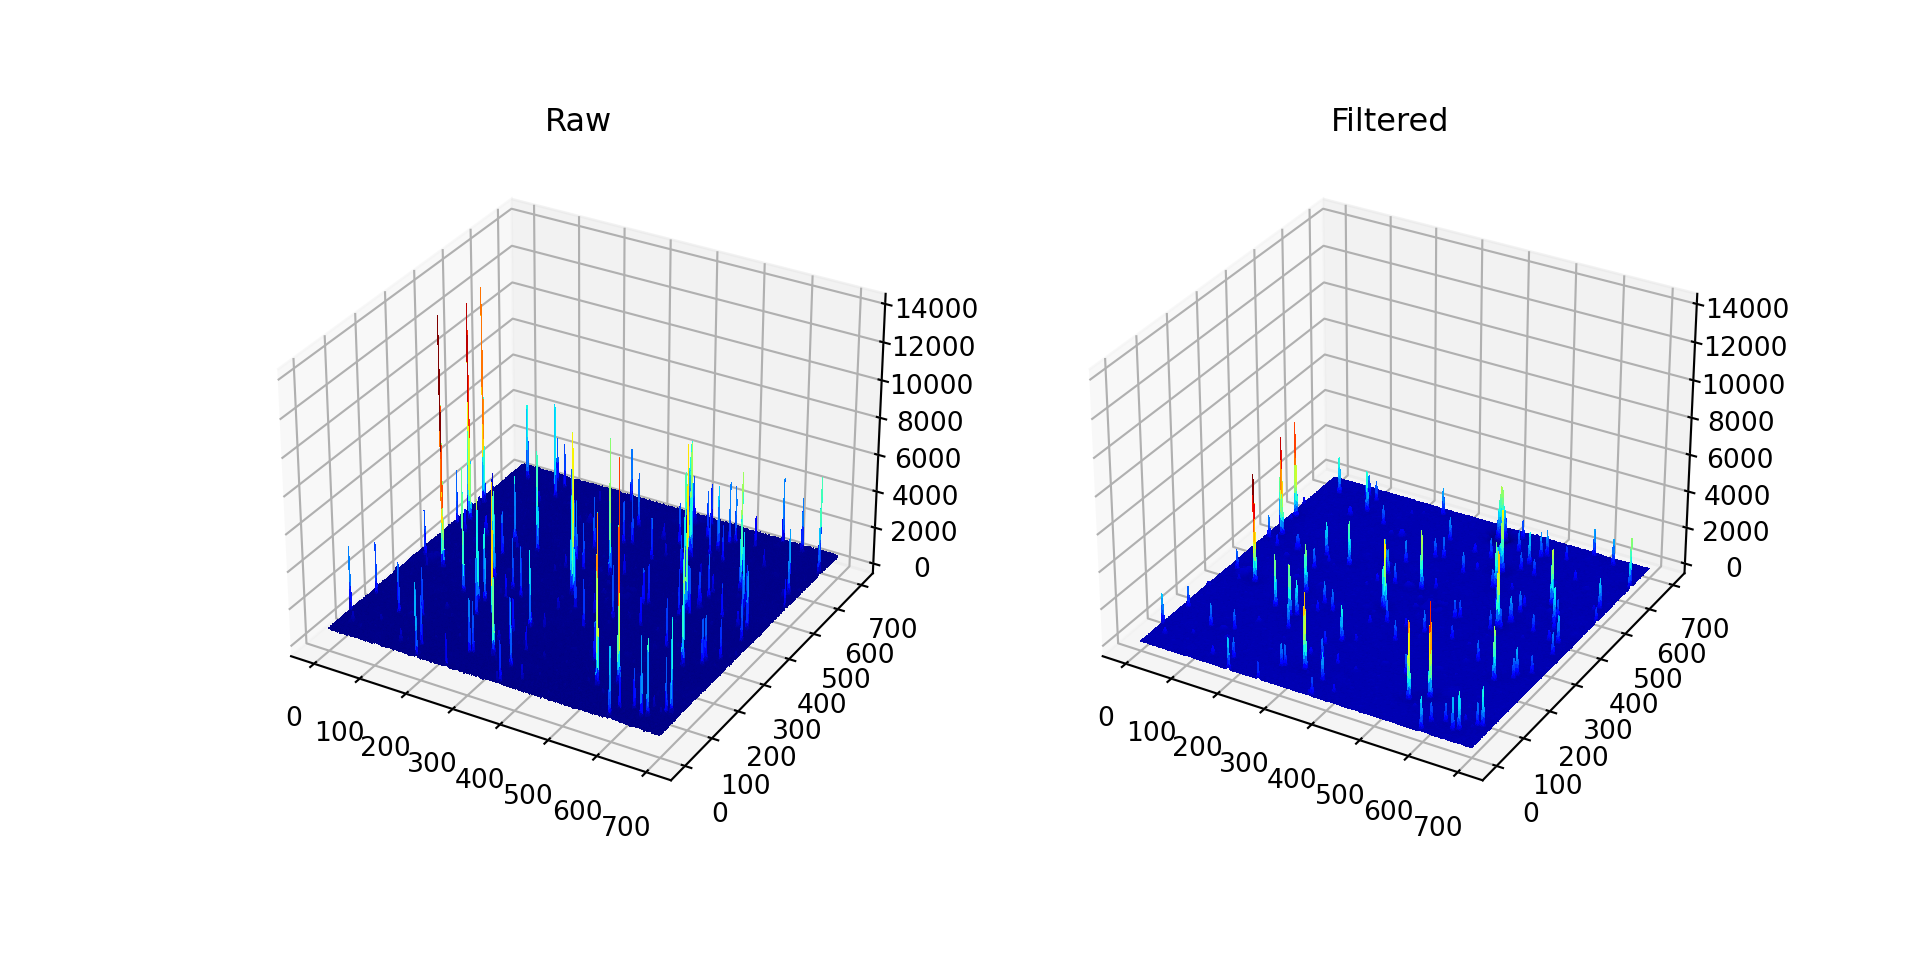
\includegraphics{Auto_files/figure-latex/unnamed-chunk-1-12.pdf}
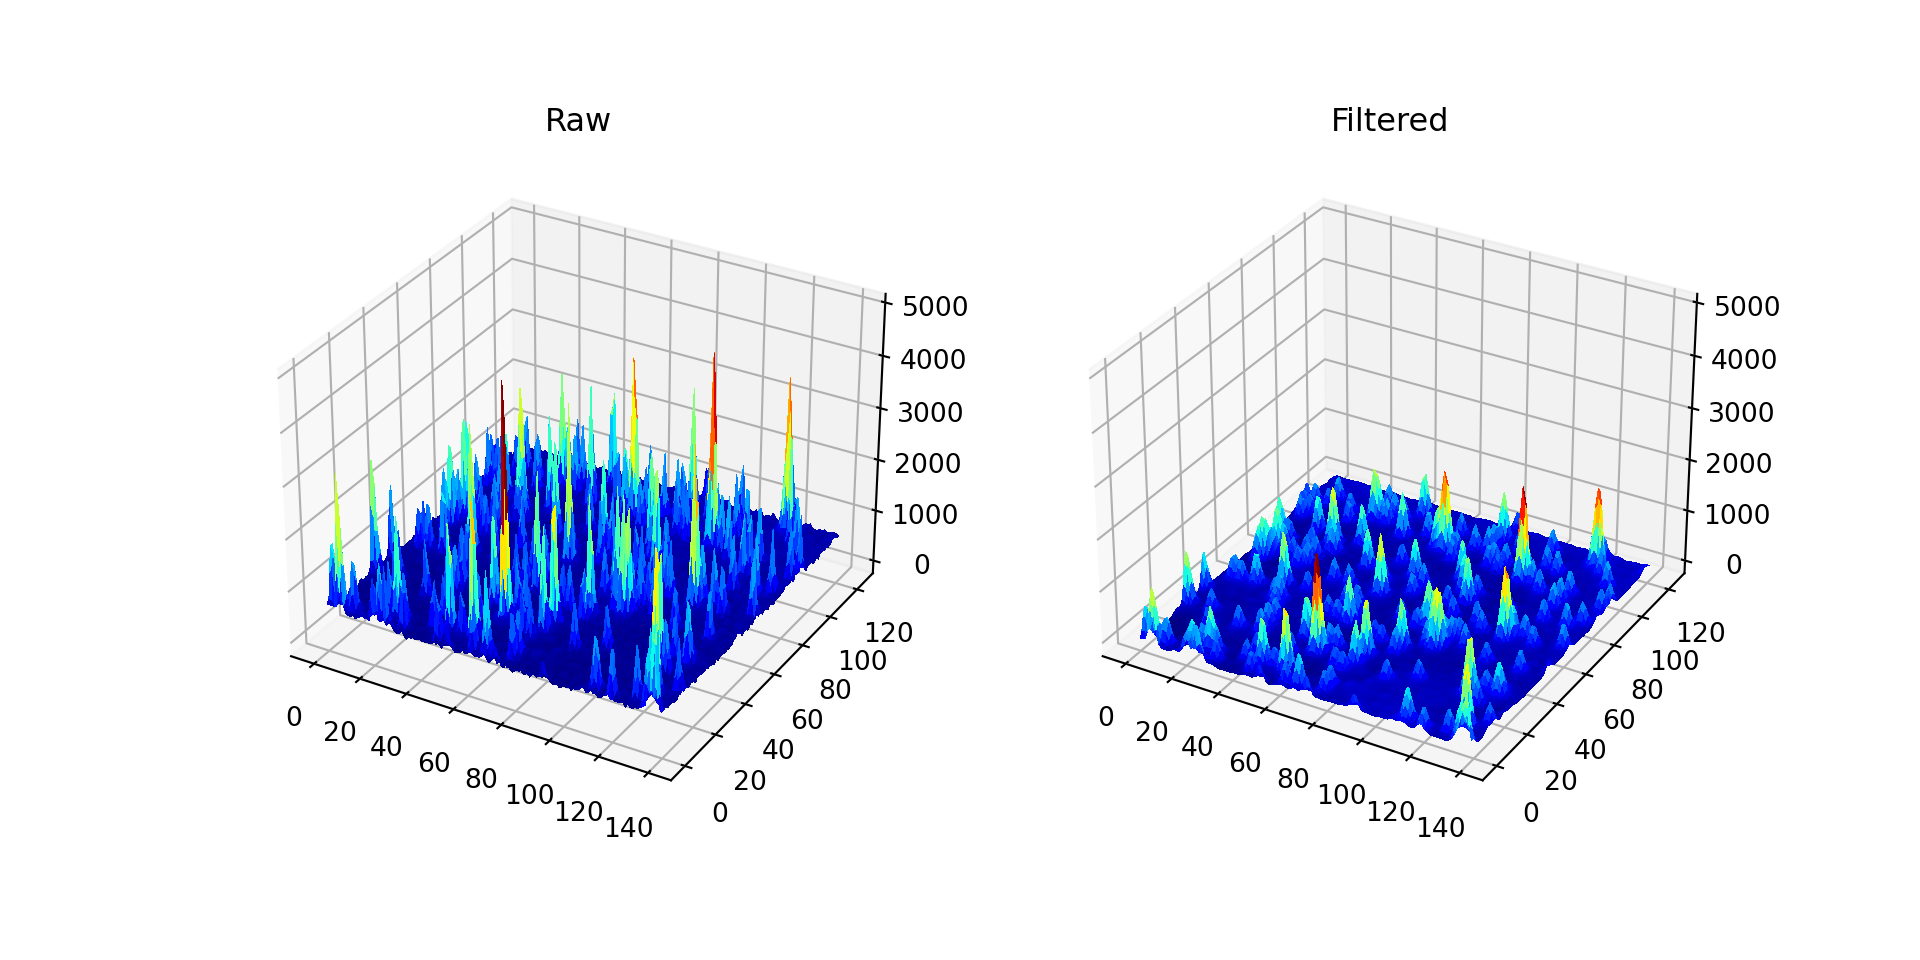
\includegraphics{Auto_files/figure-latex/unnamed-chunk-1-13.pdf}

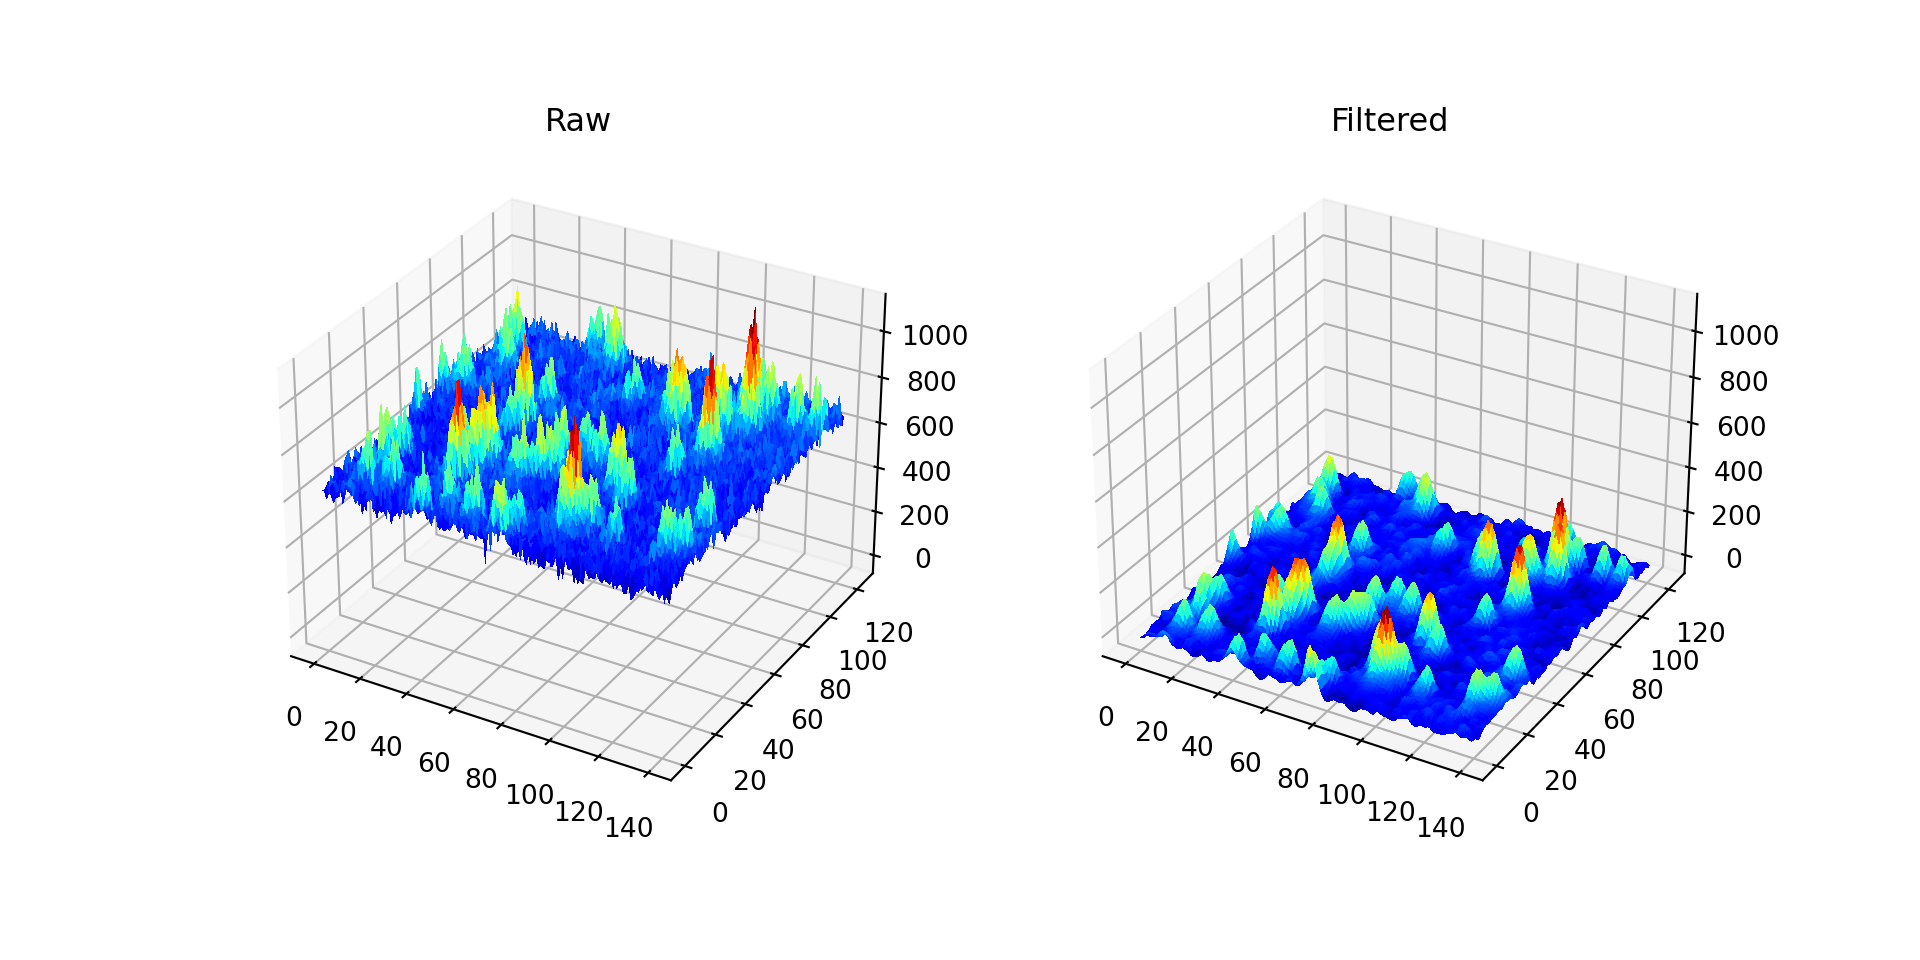
\includegraphics{Auto_files/figure-latex/unnamed-chunk-1-25.pdf}
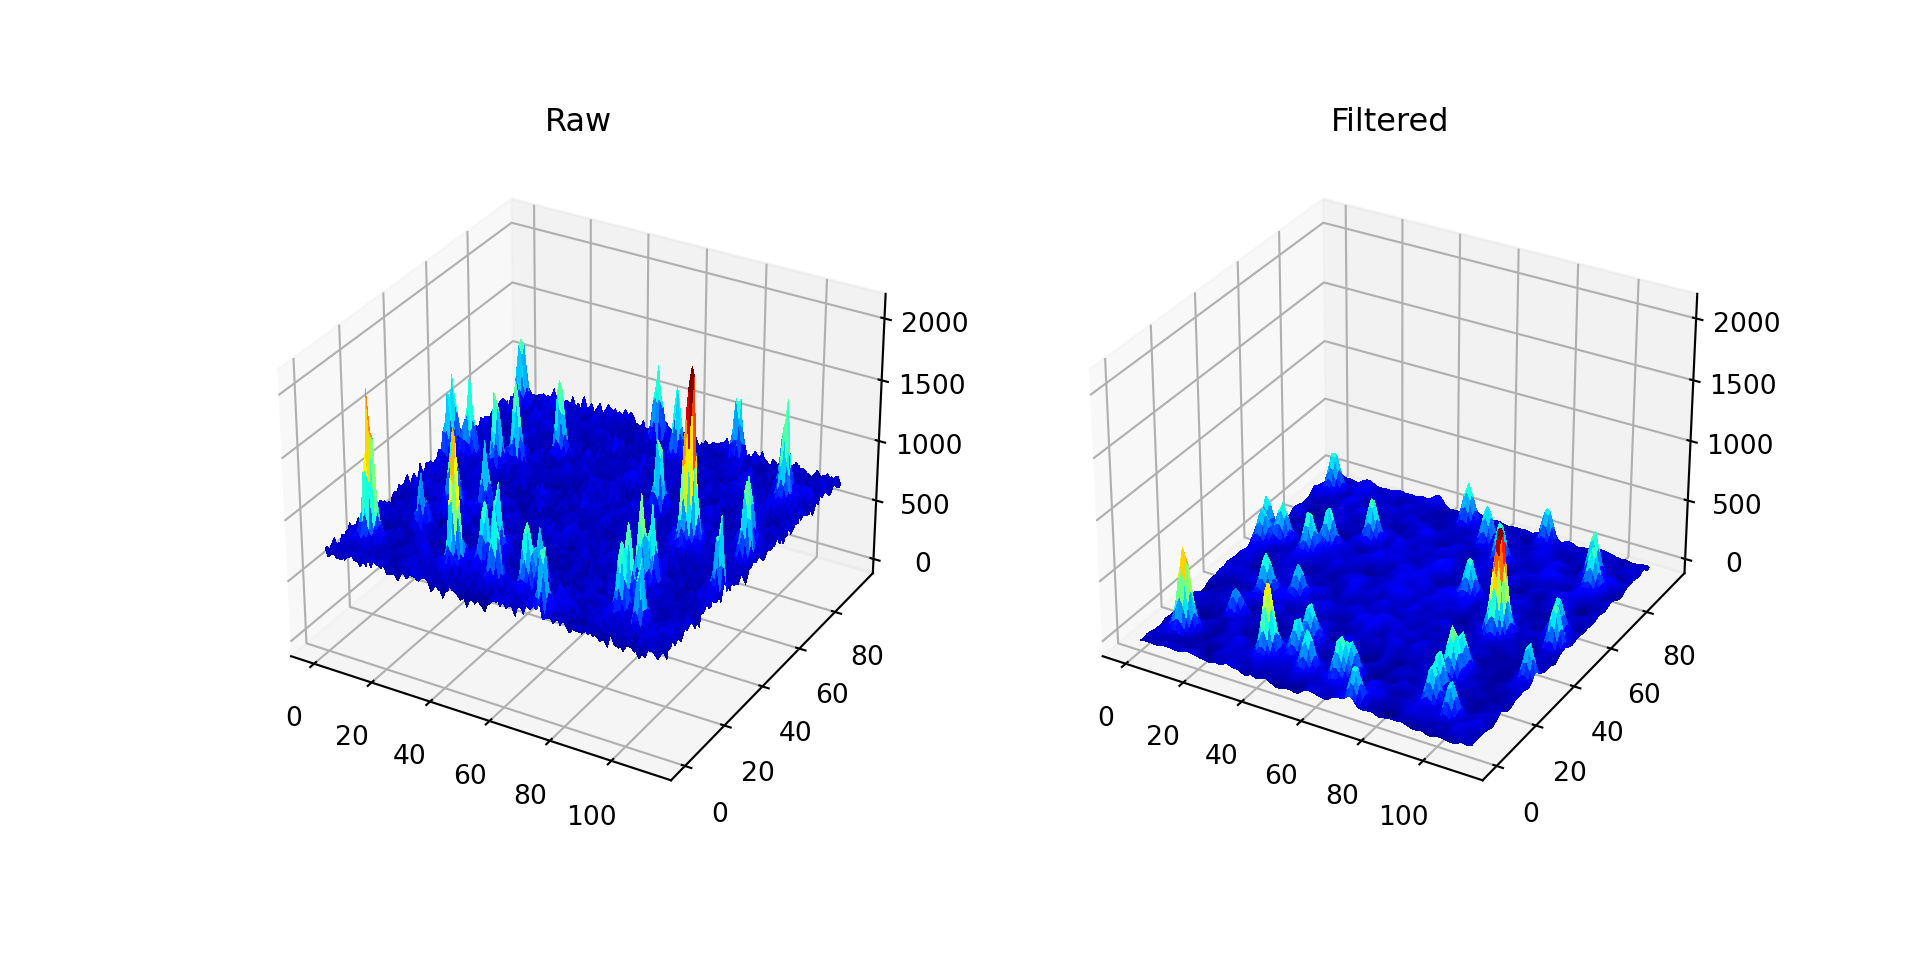
\includegraphics{Auto_files/figure-latex/unnamed-chunk-1-26.pdf}
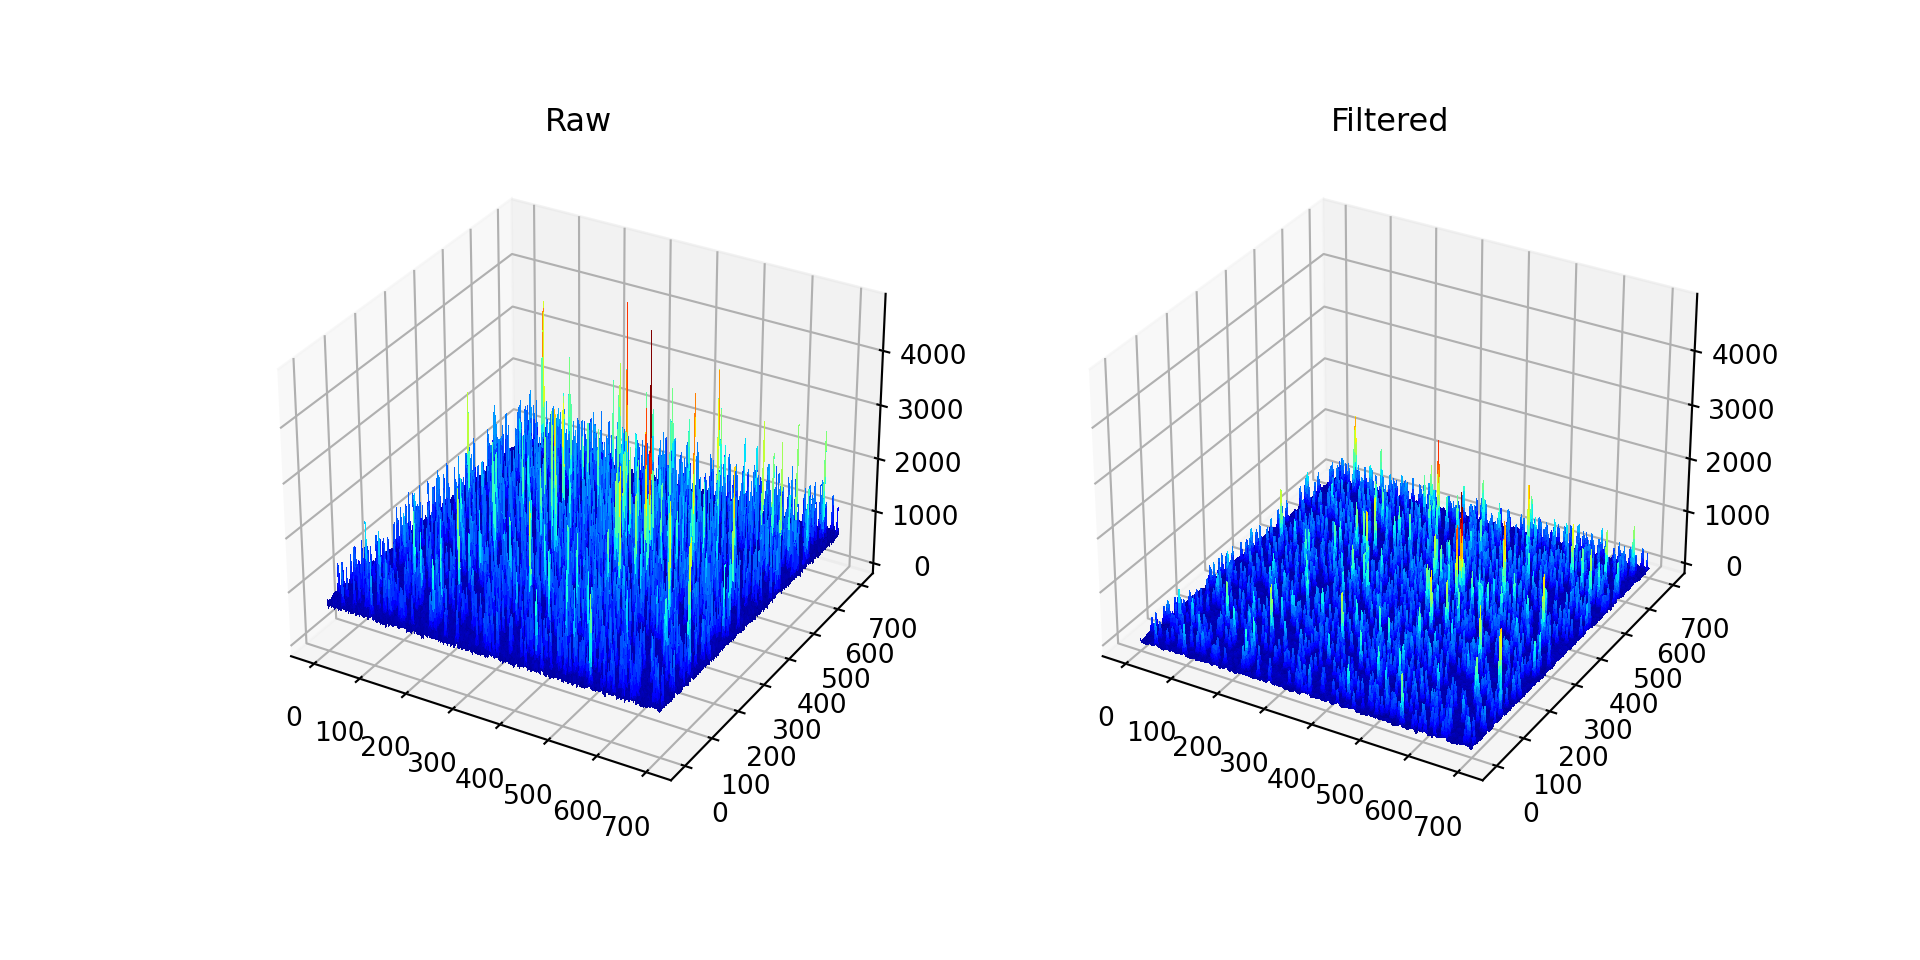
\includegraphics{Auto_files/figure-latex/unnamed-chunk-1-27.pdf}
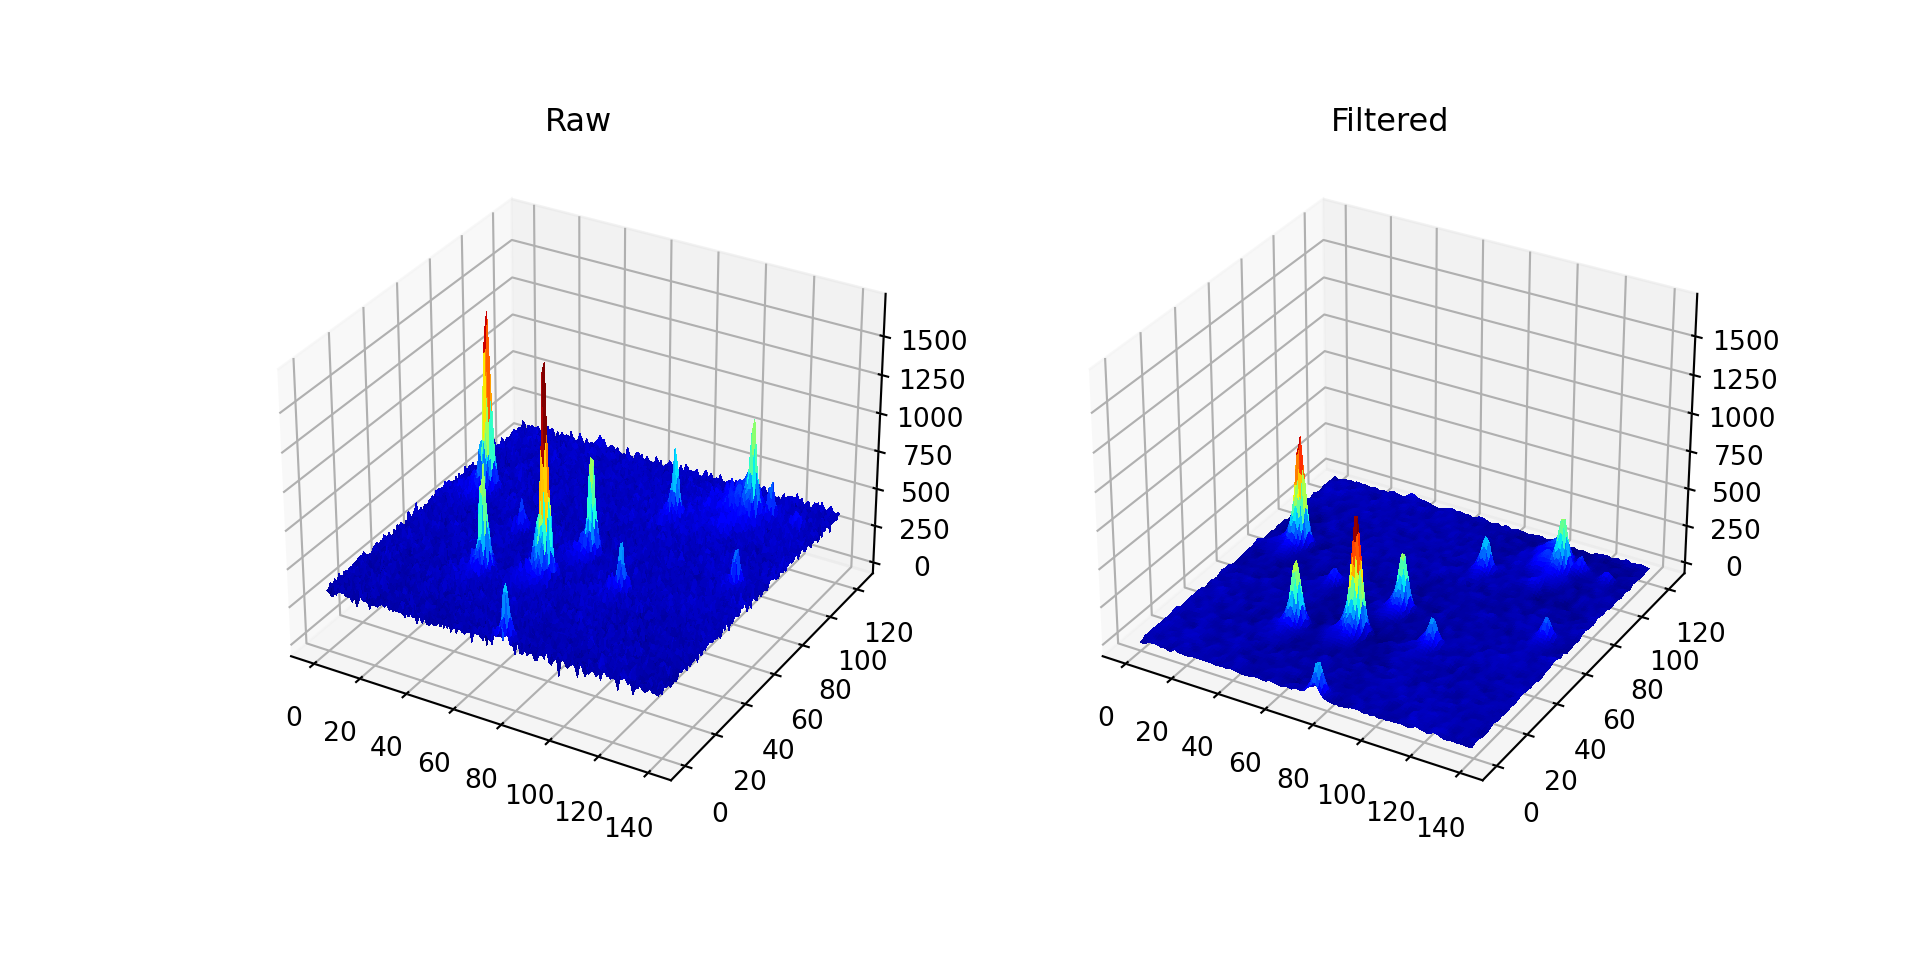
\includegraphics{Auto_files/figure-latex/unnamed-chunk-1-28.pdf}
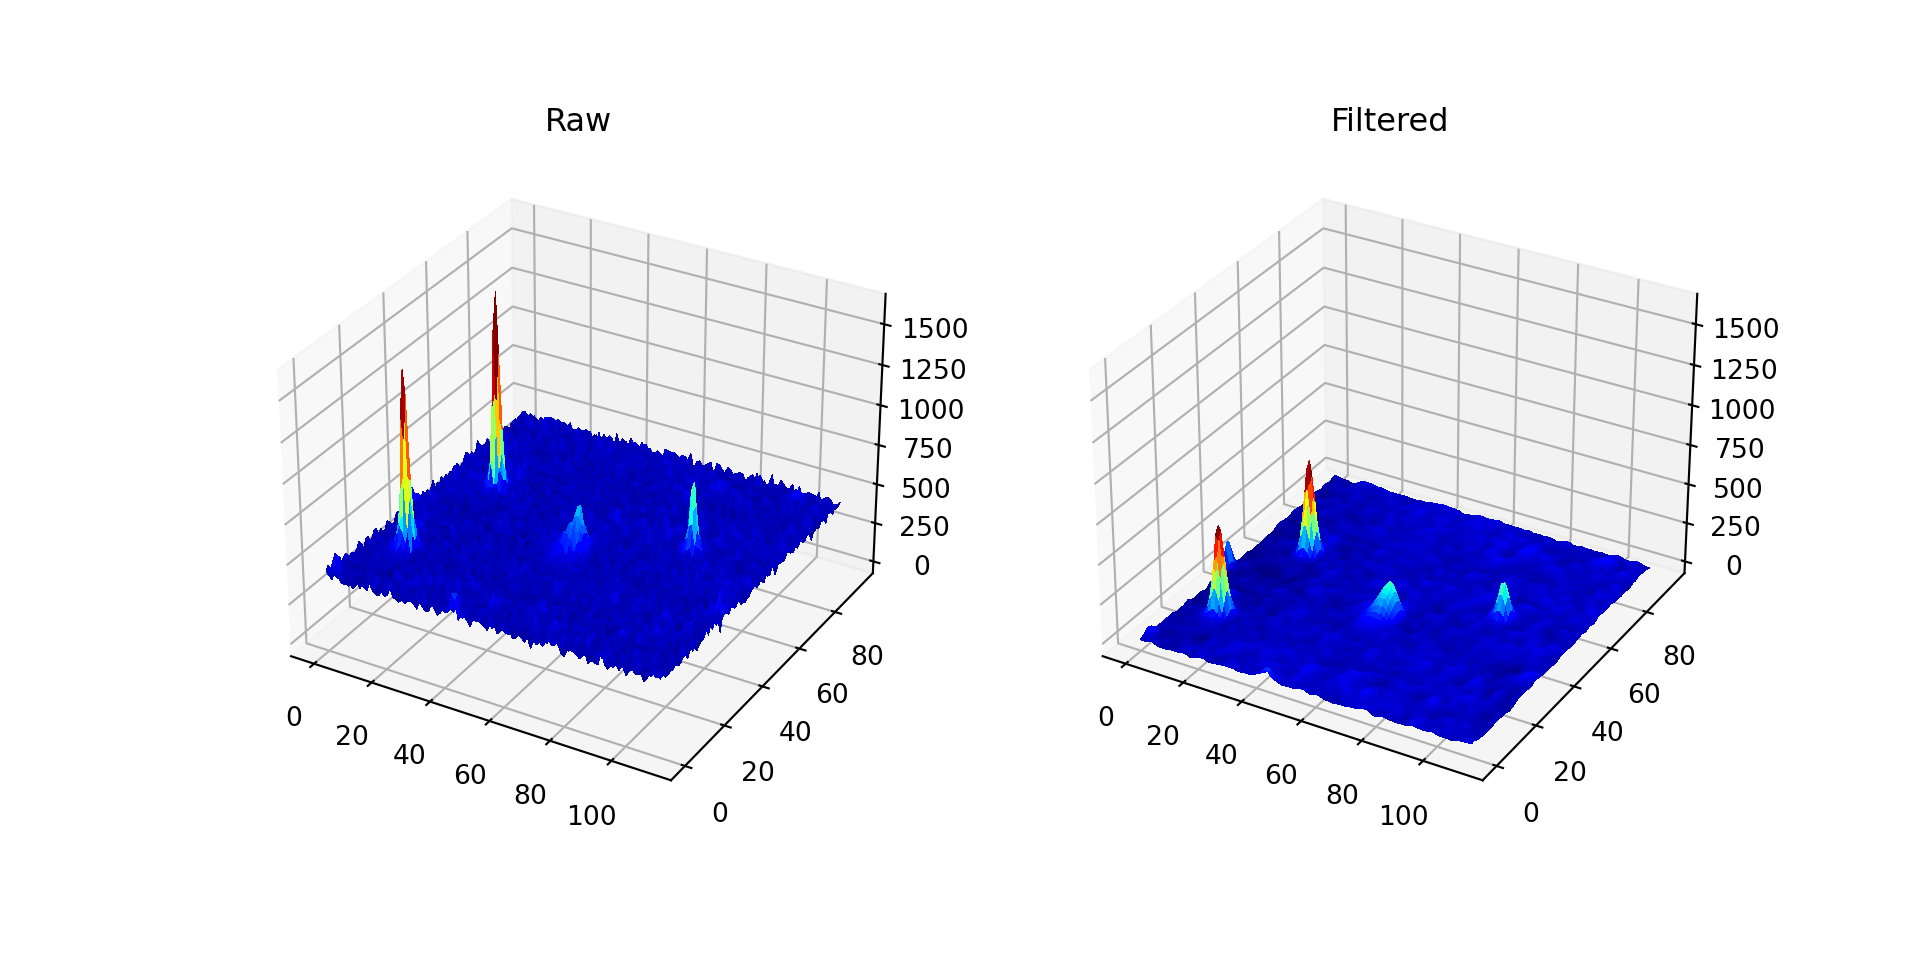
\includegraphics{Auto_files/figure-latex/unnamed-chunk-1-29.pdf}
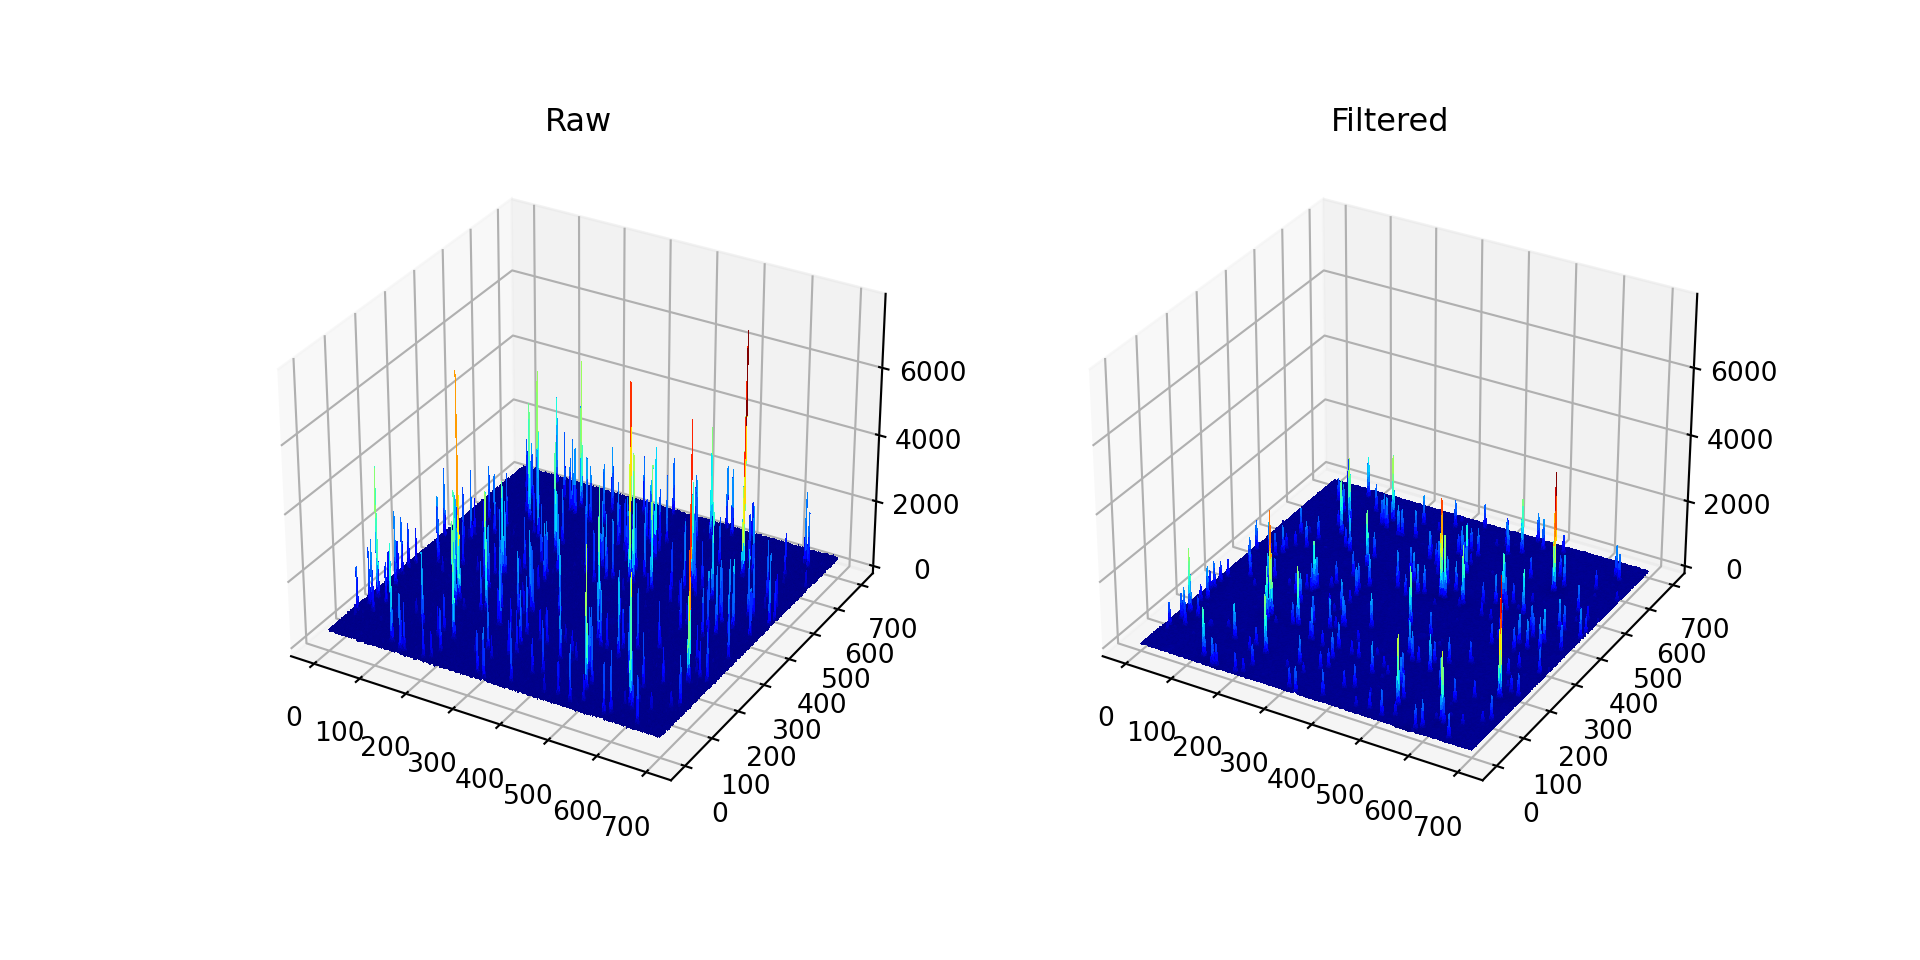
\includegraphics{Auto_files/figure-latex/unnamed-chunk-1-30.pdf}
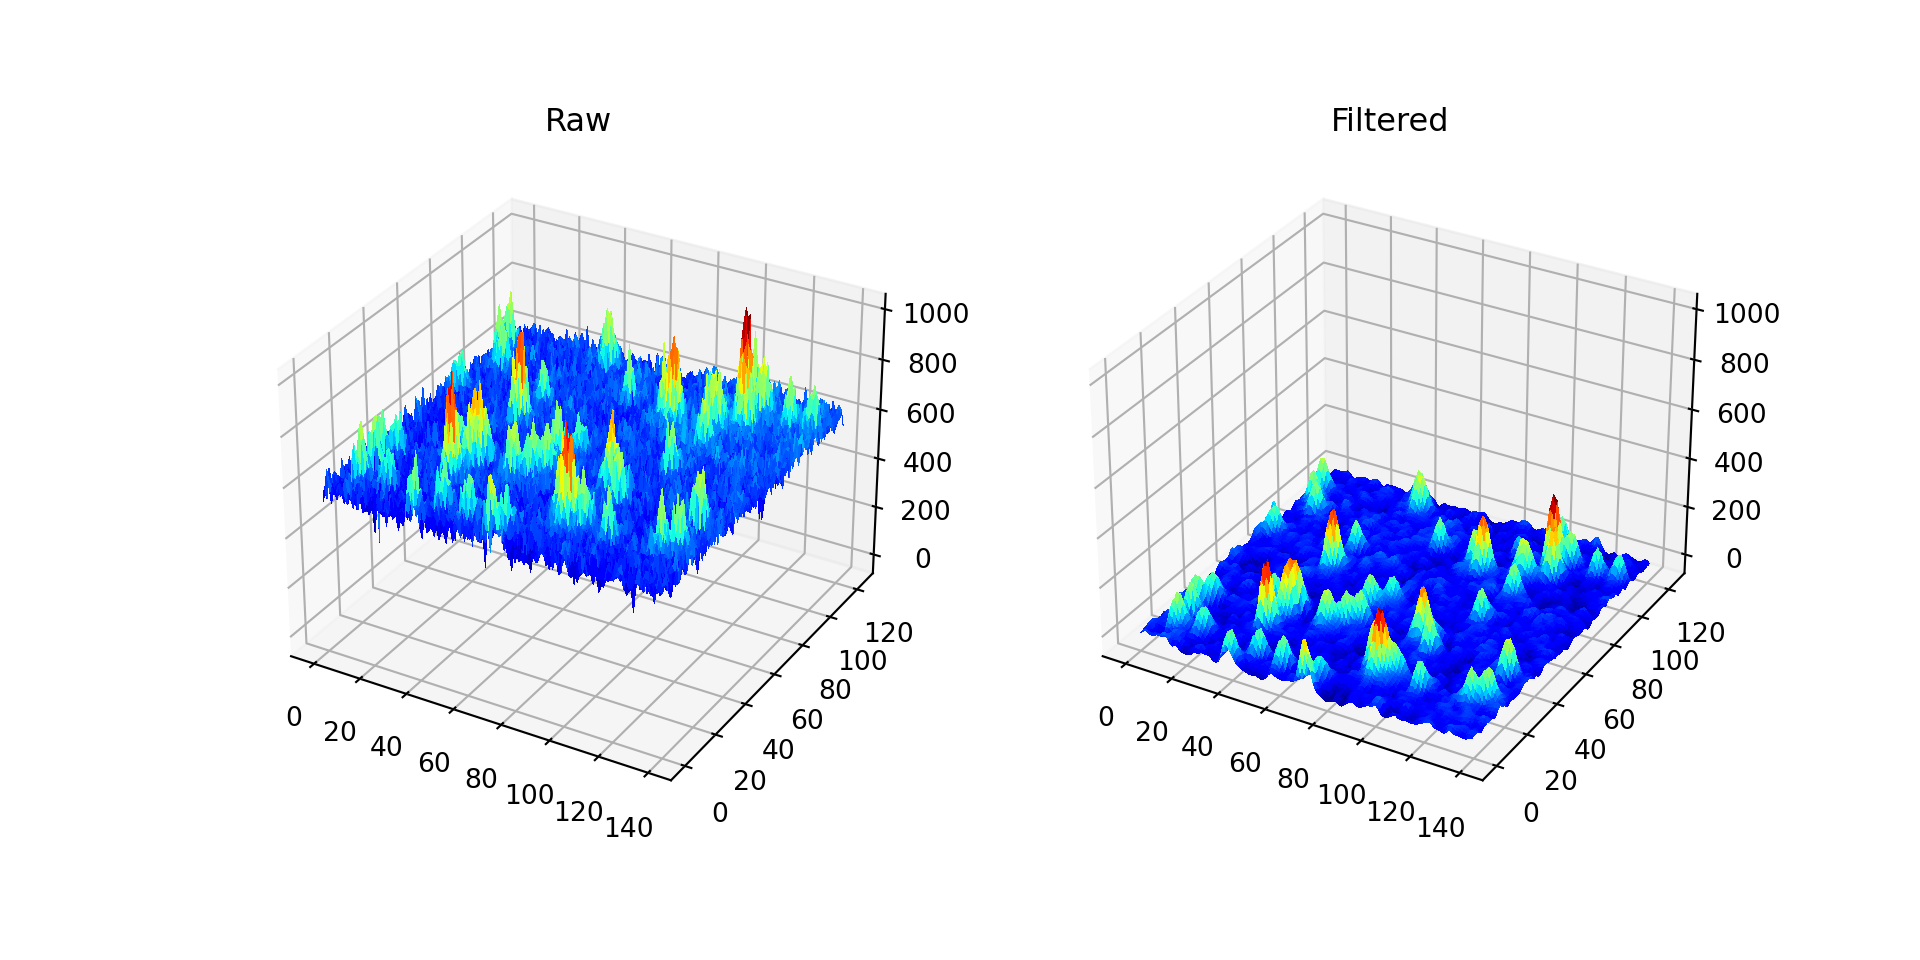
\includegraphics{Auto_files/figure-latex/unnamed-chunk-1-31.pdf}
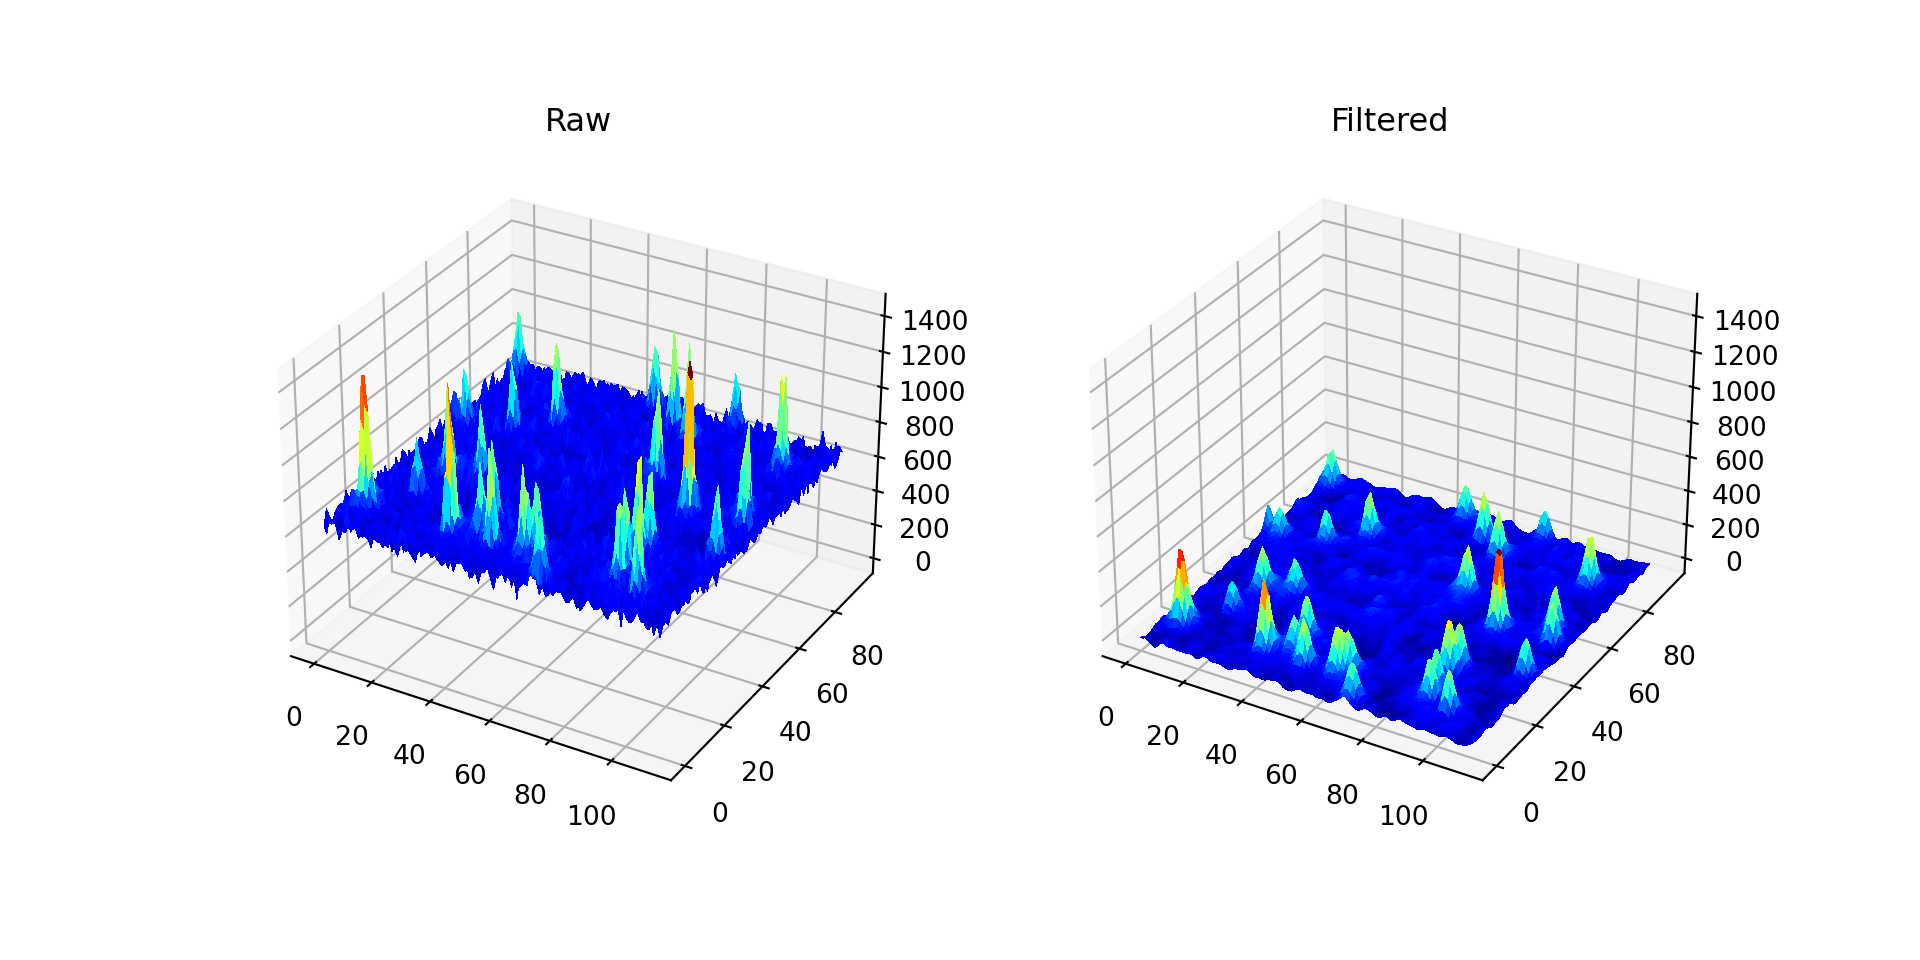
\includegraphics{Auto_files/figure-latex/unnamed-chunk-1-32.pdf}
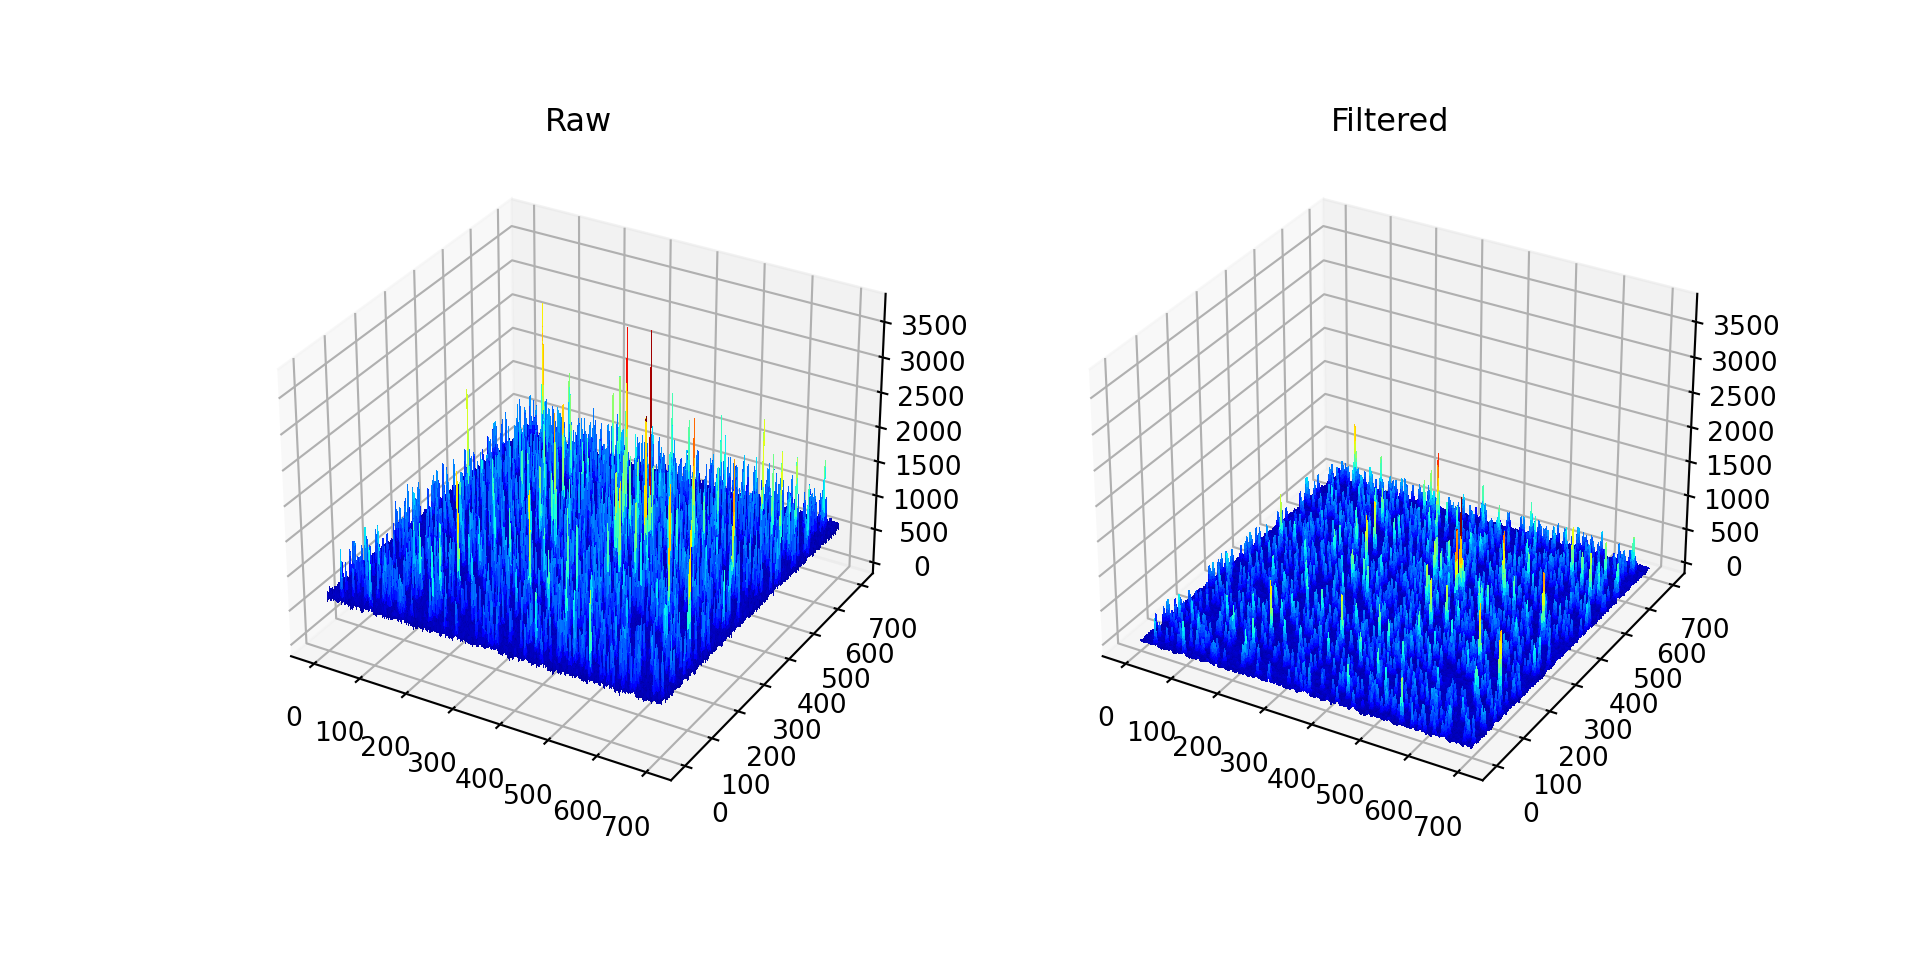
\includegraphics{Auto_files/figure-latex/unnamed-chunk-1-33.pdf}
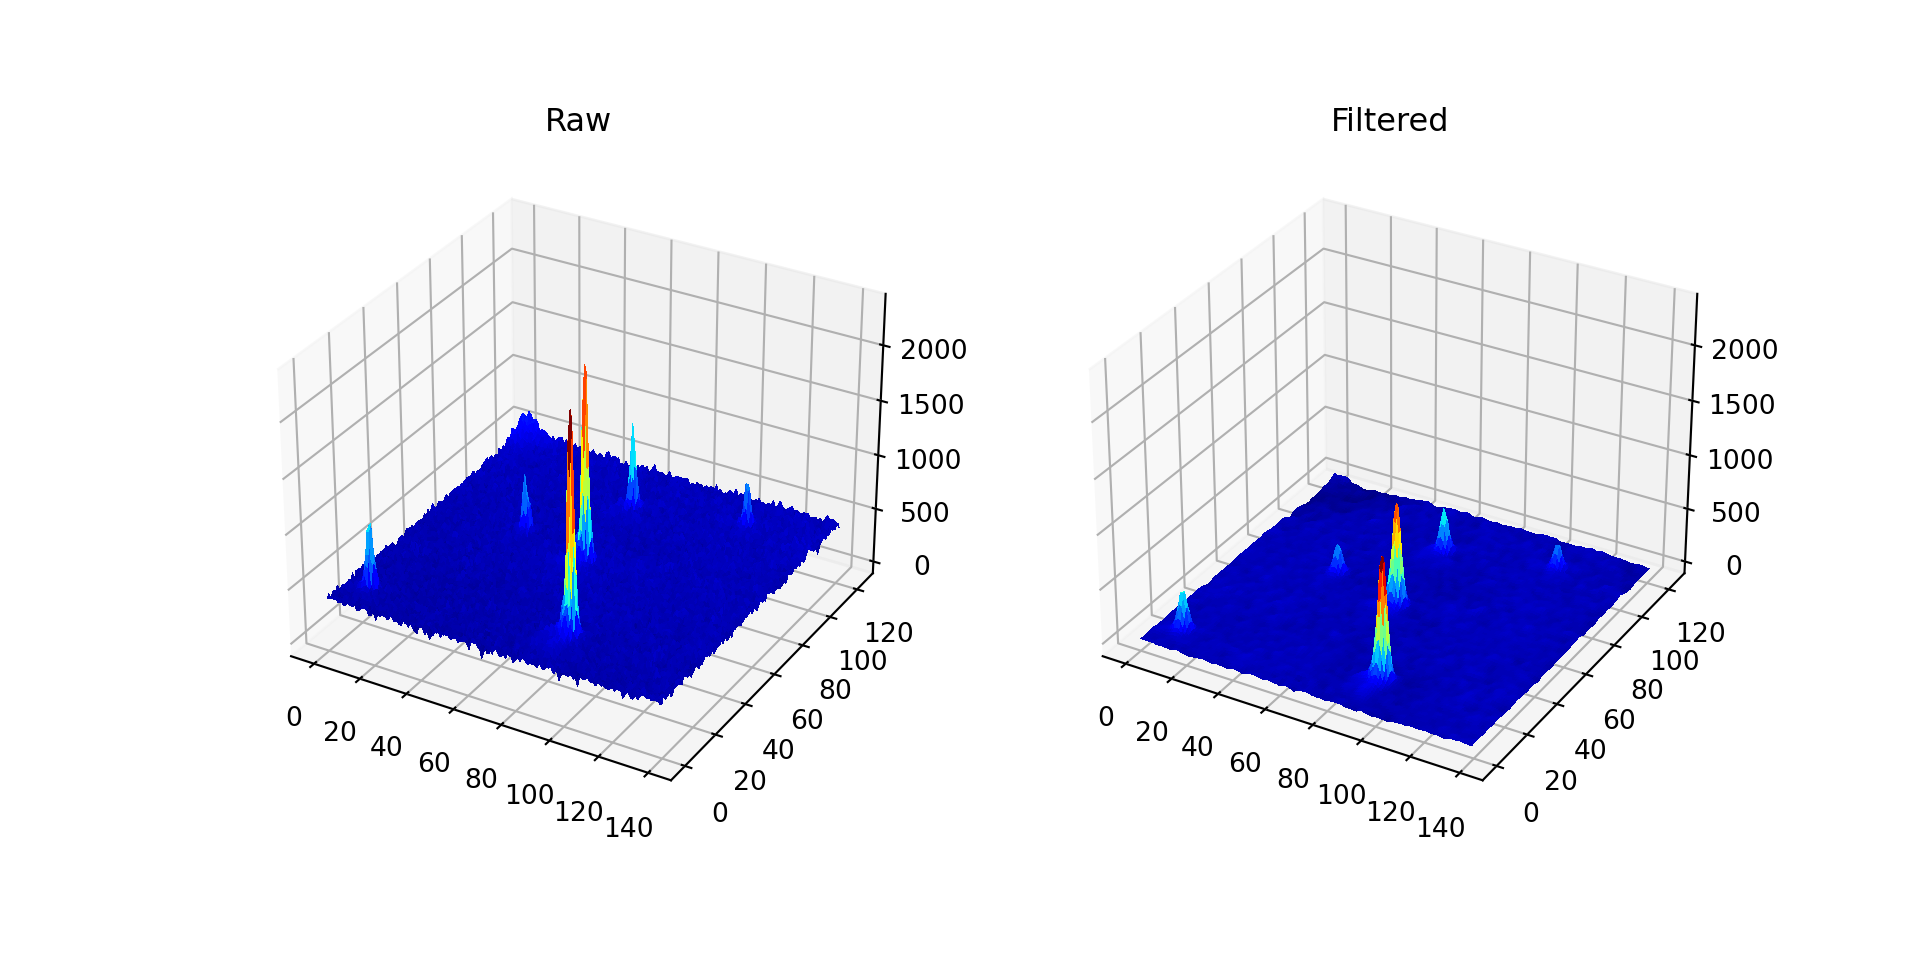
\includegraphics{Auto_files/figure-latex/unnamed-chunk-1-34.pdf}
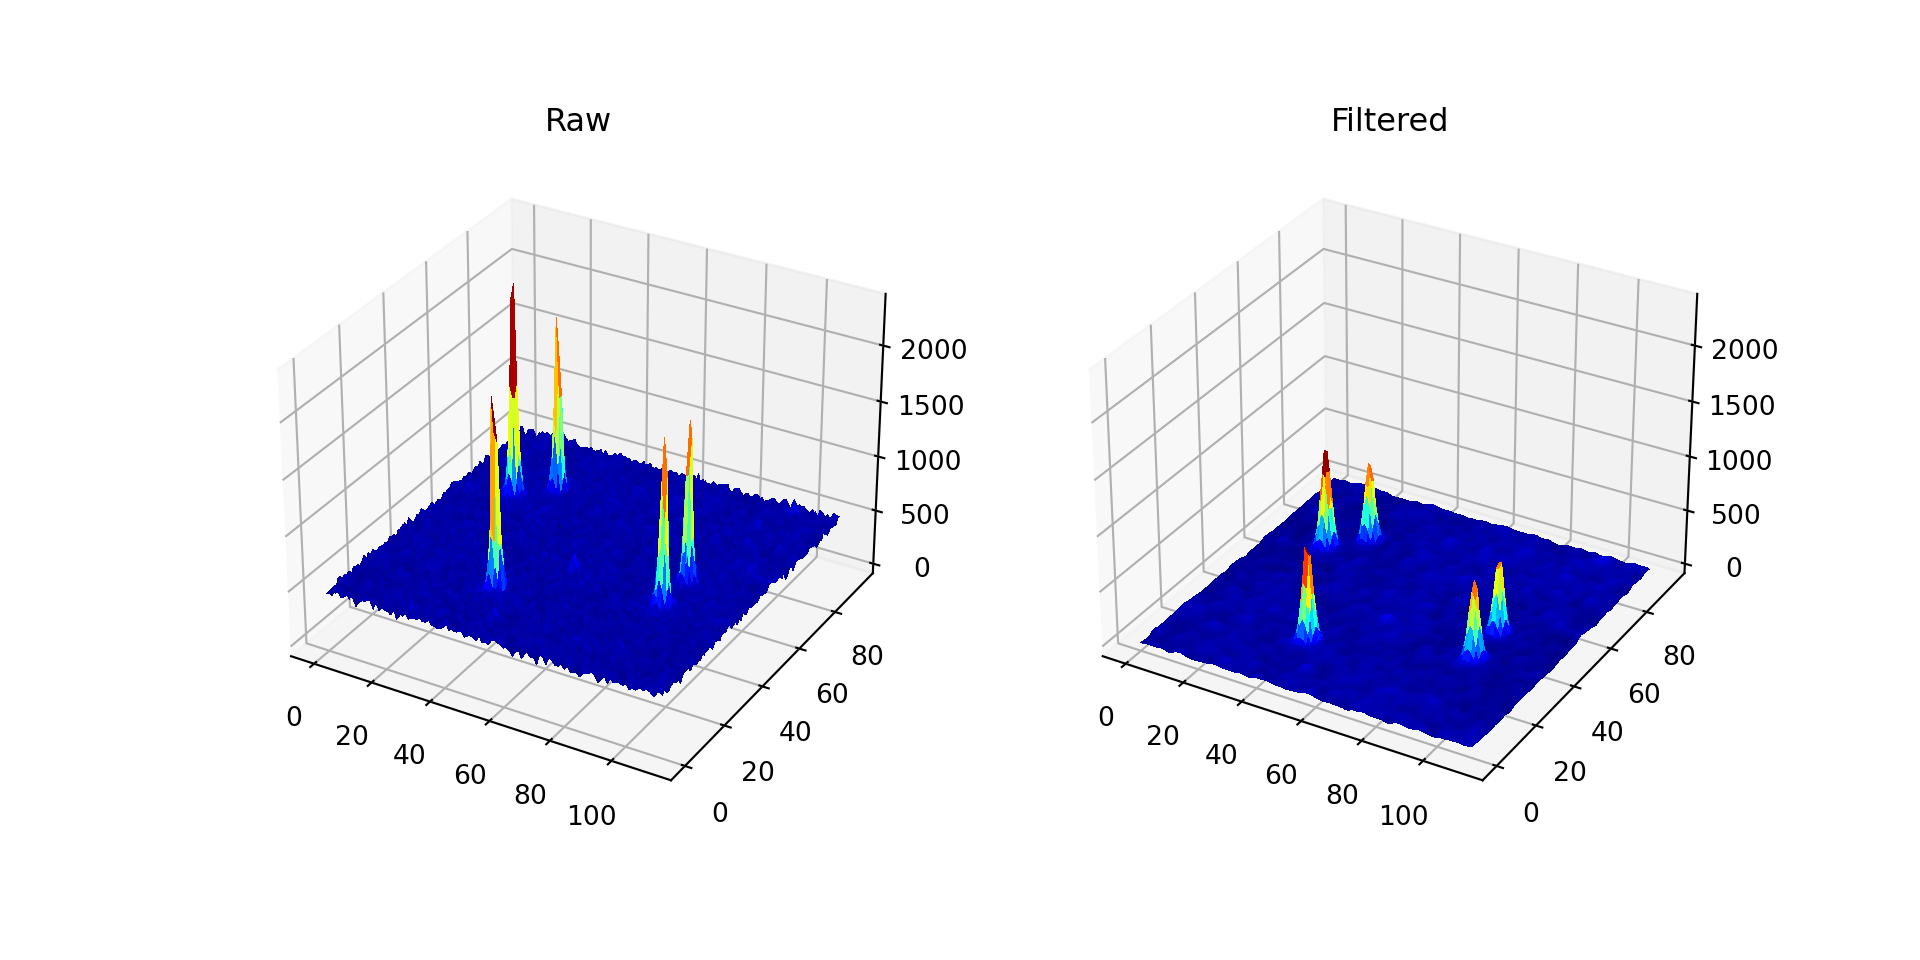
\includegraphics{Auto_files/figure-latex/unnamed-chunk-1-35.pdf}

\includegraphics{Auto_files/figure-latex/unnamed-chunk-1-47.pdf}
\includegraphics{Auto_files/figure-latex/unnamed-chunk-1-48.pdf}

\end{document}
